\documentclass[aspectratio=169,9pt]{beamer}
% Shared look for Laile's submission documents. Build with Tectonic (see submission/build.sh).
\usepackage{fontspec}
\usepackage{xcolor}
\usepackage{graphicx}
\usepackage{tikz}
\usetikzlibrary{positioning,fit,backgrounds,arrows.meta,calc,shapes.misc}

% macOS system fonts: Avenir Next for text, Hiragino Sans GB for 莱乐.
\setmainfont{Avenir Next.ttc}[
  Path=/System/Library/Fonts/,
  UprightFeatures={FontIndex=7},
  BoldFont={Avenir Next.ttc}, BoldFeatures={FontIndex=2},
  ItalicFont={Avenir Next.ttc}, ItalicFeatures={FontIndex=4},
  BoldItalicFont={Avenir Next.ttc}, BoldItalicFeatures={FontIndex=3}]
\setsansfont{Avenir Next.ttc}[
  Path=/System/Library/Fonts/,
  UprightFeatures={FontIndex=7},
  BoldFont={Avenir Next.ttc}, BoldFeatures={FontIndex=2},
  ItalicFont={Avenir Next.ttc}, ItalicFeatures={FontIndex=4},
  BoldItalicFont={Avenir Next.ttc}, BoldItalicFeatures={FontIndex=3}]
\newfontfamily\heavyfont{Avenir Next.ttc}[Path=/System/Library/Fonts/, UprightFeatures={FontIndex=8}]
\newfontfamily\cjk{Hiragino Sans GB.ttc}[Path=/System/Library/Fonts/, UprightFeatures={FontIndex=2}]

% The app's palette (DesignSystem/Theme.swift).
\definecolor{accent}{HTML}{0F8A6A}
\definecolor{accentsoft}{HTML}{DFF3EC}
\definecolor{reward}{HTML}{E8930C}
\definecolor{rewardsoft}{HTML}{FFF1DC}
\definecolor{danger}{HTML}{C62828}
\definecolor{dangersoft}{HTML}{FDE7E5}
\definecolor{ink}{HTML}{17211C}
\definecolor{muted}{HTML}{5D6B63}
\definecolor{surface}{HTML}{EEF2EF}
\definecolor{paper}{HTML}{F6F7F5}

\newcommand{\laile}{Laile ({\cjk 莱乐})}
\newcommand{\lele}{Lele ({\cjk 乐乐})}
\newcommand{\wordmark}{{\cjk\color{accent}莱乐}}

\usepackage{booktabs}
\usepackage{tabularx}

% ---- Look ---------------------------------------------------------------
\setbeamertemplate{navigation symbols}{}
\setbeamercolor{background canvas}{bg=paper}
\setbeamercolor{normal text}{fg=ink}
\setbeamercolor{frametitle}{fg=ink}
\setbeamercolor{structure}{fg=accent}
\setbeamercolor{itemize item}{fg=accent}
\setbeamerfont{frametitle}{size=\LARGE,series=\bfseries}
\setbeamertemplate{frametitle}{\vspace{10pt}\insertframetitle\par\vspace{2pt}{\color{accent}\rule{1.2cm}{2pt}}}
\setbeamertemplate{itemize items}{\raisebox{1pt}{\color{accent}\rule{5pt}{5pt}}}
\setbeamertemplate{footline}{\hfill{\scriptsize\color{muted}\laile\quad\insertframenumber\hspace{14pt}}\vspace{8pt}}
\setlength{\parskip}{4pt}

\newcommand{\phone}[2][0.17]{\begin{minipage}[t]{#1\linewidth}\centering
  \includegraphics[width=\linewidth]{../screenshots/#2}\end{minipage}}
\newcommand{\capt}[1]{{\scriptsize\color{muted}#1}}
\newcommand{\bignum}[1]{{\fontsize{30}{32}\selectfont\bfseries\color{accent}#1}}
\newcommand{\pill}[1]{\tikz[baseline=(p.base)]\node[fill=accentsoft,text=accent,rounded corners=6pt,inner sep=3pt,font=\scriptsize\bfseries](p){#1};}

\begin{document}

% ---- 1. Title -----------------------------------------------------------
{\setbeamertemplate{footline}{}
\begin{frame}
\begin{columns}[c]
\begin{column}{0.56\textwidth}
  
\includegraphics[height=3.2cm]{../brand/lockup-transparent.png}\\[10pt]
  {\Large Home physio that counts every rep and checks in.}\\[18pt]
  {\small\color{muted}Tencent Cloud AI CAN DO IT Hackathon Singapore 2026\\
  Healthcare track \textbullet\ Challenge Statement 2\\[4pt]
  Charles Andrew Lim}
\end{column}
\begin{column}{0.4\textwidth}\centering
  \phone[0.42]{02-today.png}\hspace{4pt}\phone[0.42]{04-lele-chat.png}
\end{column}
\end{columns}
\end{frame}}

% ---- 2. Problem ---------------------------------------------------------
\begin{frame}{Physio happens at home, where nobody sees it}
\begin{columns}[t]
\begin{column}{0.32\textwidth}
  \bignum{50\%}\\[2pt]
  of people in rehab may not do their home exercise [1]\\[10pt]
  \bignum{21.4\%}\\[2pt]
  of Singapore citizens are 65 or older (2026), a super-aged society [3]
\end{column}
\begin{column}{0.64\textwidth}
  \textbf{Why people stop} (systematic review of 20 studies [2]):
  low confidence, low mood, worry, pain during exercise, no support, too many barriers.\\[6pt]
  \textbf{What a physio sees between visits:} nothing. A checkbox can't tell a done exercise from a skipped one, or one stopped because it hurt.\\[6pt]
  \textbf{What the brief asks for:} support that is empowering, personalised, longitudinal, safe, strictly bounded and honest about uncertainty.
\end{column}
\end{columns}
\end{frame}

% ---- 3. Idea ------------------------------------------------------------
\begin{frame}{Laile in one breath}
\begin{columns}[c]
\begin{column}{0.6\textwidth}
\begin{itemize}
  \item \textbf{Programs are the unit.} A physio's program (joined with their code), a plan Lele builds from your goals, or a calisthenics program.
  \item \textbf{The camera counts.} Reps, holds, knee bend and arm lift, measured on the phone. Video stays there.
  \item \textbf{Lele checks in.} A coach that talks you through sessions, asks how you are each morning, reminds, notices, remembers what hurt.
  \item \textbf{The physio stays on top.} Live sessions, a daily list, approvals, signatures, discharge.
  \item \textbf{Code decides, the model talks.} Safety and every number come from tested rules.
  \item \textbf{iPhone or any browser.} Same account, same sessions, same Lele.
\end{itemize}
\end{column}
\begin{column}{0.36\textwidth}\centering
  \phone[0.42]{08-session.png}\hspace{4pt}\phone[0.42]{03-lele-inbox.png}
\end{column}
\end{columns}
\end{frame}

% ---- 4. Start ----------------------------------------------------------
\begin{frame}{Start: tell Lele your goals, or bring a physio's code}
\centering
\phone{12-goals-conversation.png}\hfill
\phone{13-plan-built.png}\hfill
\phone{09-targets-set.png}\hfill
\phone{14-precautions-follow.png}\\[4pt]
\begin{minipage}[t]{0.205\linewidth}\centering\capt{Goals in your own words; options are suggestions}\end{minipage}\hfill
\begin{minipage}[t]{0.205\linewidth}\centering\capt{Lele's plan leaves out what your wrists can't take}\end{minipage}\hfill
\begin{minipage}[t]{0.205\linewidth}\centering\capt{First session is a check-in that sets targets}\end{minipage}\hfill
\begin{minipage}[t]{0.205\linewidth}\centering\capt{Limits follow you into every program}\end{minipage}
\end{frame}

% ---- 5. Sessions ---------------------------------------------------------
\begin{frame}{Sessions: the camera counts, Lele coaches}
\begin{columns}[c]
\begin{column}{0.3\textwidth}\centering
  \phone[0.62]{08-session.png}
\end{column}
\begin{column}{0.66\textwidth}
\begin{itemize}
  \item Apple Vision on iPhone, MediaPipe in the browser: joints are tracked on the device; a rep counts only at the target angle, a hold only while in position.
  \item Lele takes turns like a conversation: explains, says \emph{``In your own time''}, counts, asks \emph{``How did that feel?''} between sets.
  \item Say ``it's pulling'' or ``sharp pain'' any time. Fixed rules decide: carry on, stop the set, stop, or get help.
  \item Something sore? Lele notes it and makes that exercise easier next time, then eases back after two comfortable sessions.
  \item Can't see you? No count: \emph{``I can't see you clearly, so I'm not counting that.''}
\end{itemize}
\end{column}
\end{columns}
\end{frame}

% ---- 6. Lele -------------------------------------------------------------
\begin{frame}{Lele takes initiative, and you can talk back}
\begin{columns}[c]
\begin{column}{0.58\textwidth}
\begin{itemize}
  \item \textbf{Morning check-in} in physio. ``Quite swollen this morning'' makes today's session gentler and tells the physio.
  \item \textbf{Medicine reminders} at the doctor's times, as notifications too; ``What's this for?'' on every dose.
  \item \textbf{Missed days:} one nudge, then ``what's getting in the way?''
  \item \textbf{Plateaus and visit prep} from real measurements.
  \item \textbf{Chat or call} Lele, built on Tencent Cloud ADP with a curated knowledge base.
  \item \textbf{Never nags:} quiet 9\,pm to 7\,am, three conversations a day at most.
\end{itemize}
\end{column}
\begin{column}{0.38\textwidth}\centering
  \phone[0.42]{03-lele-inbox.png}\hspace{4pt}\phone[0.42]{04-lele-chat.png}
\end{column}
\end{columns}
\end{frame}

% ---- 6b. Plan with Lele ---------------------------------------------------
\begin{frame}{Talk to Lele to change your goals}
\begin{columns}[c]
\begin{column}{0.5\textwidth}\centering
  \fbox{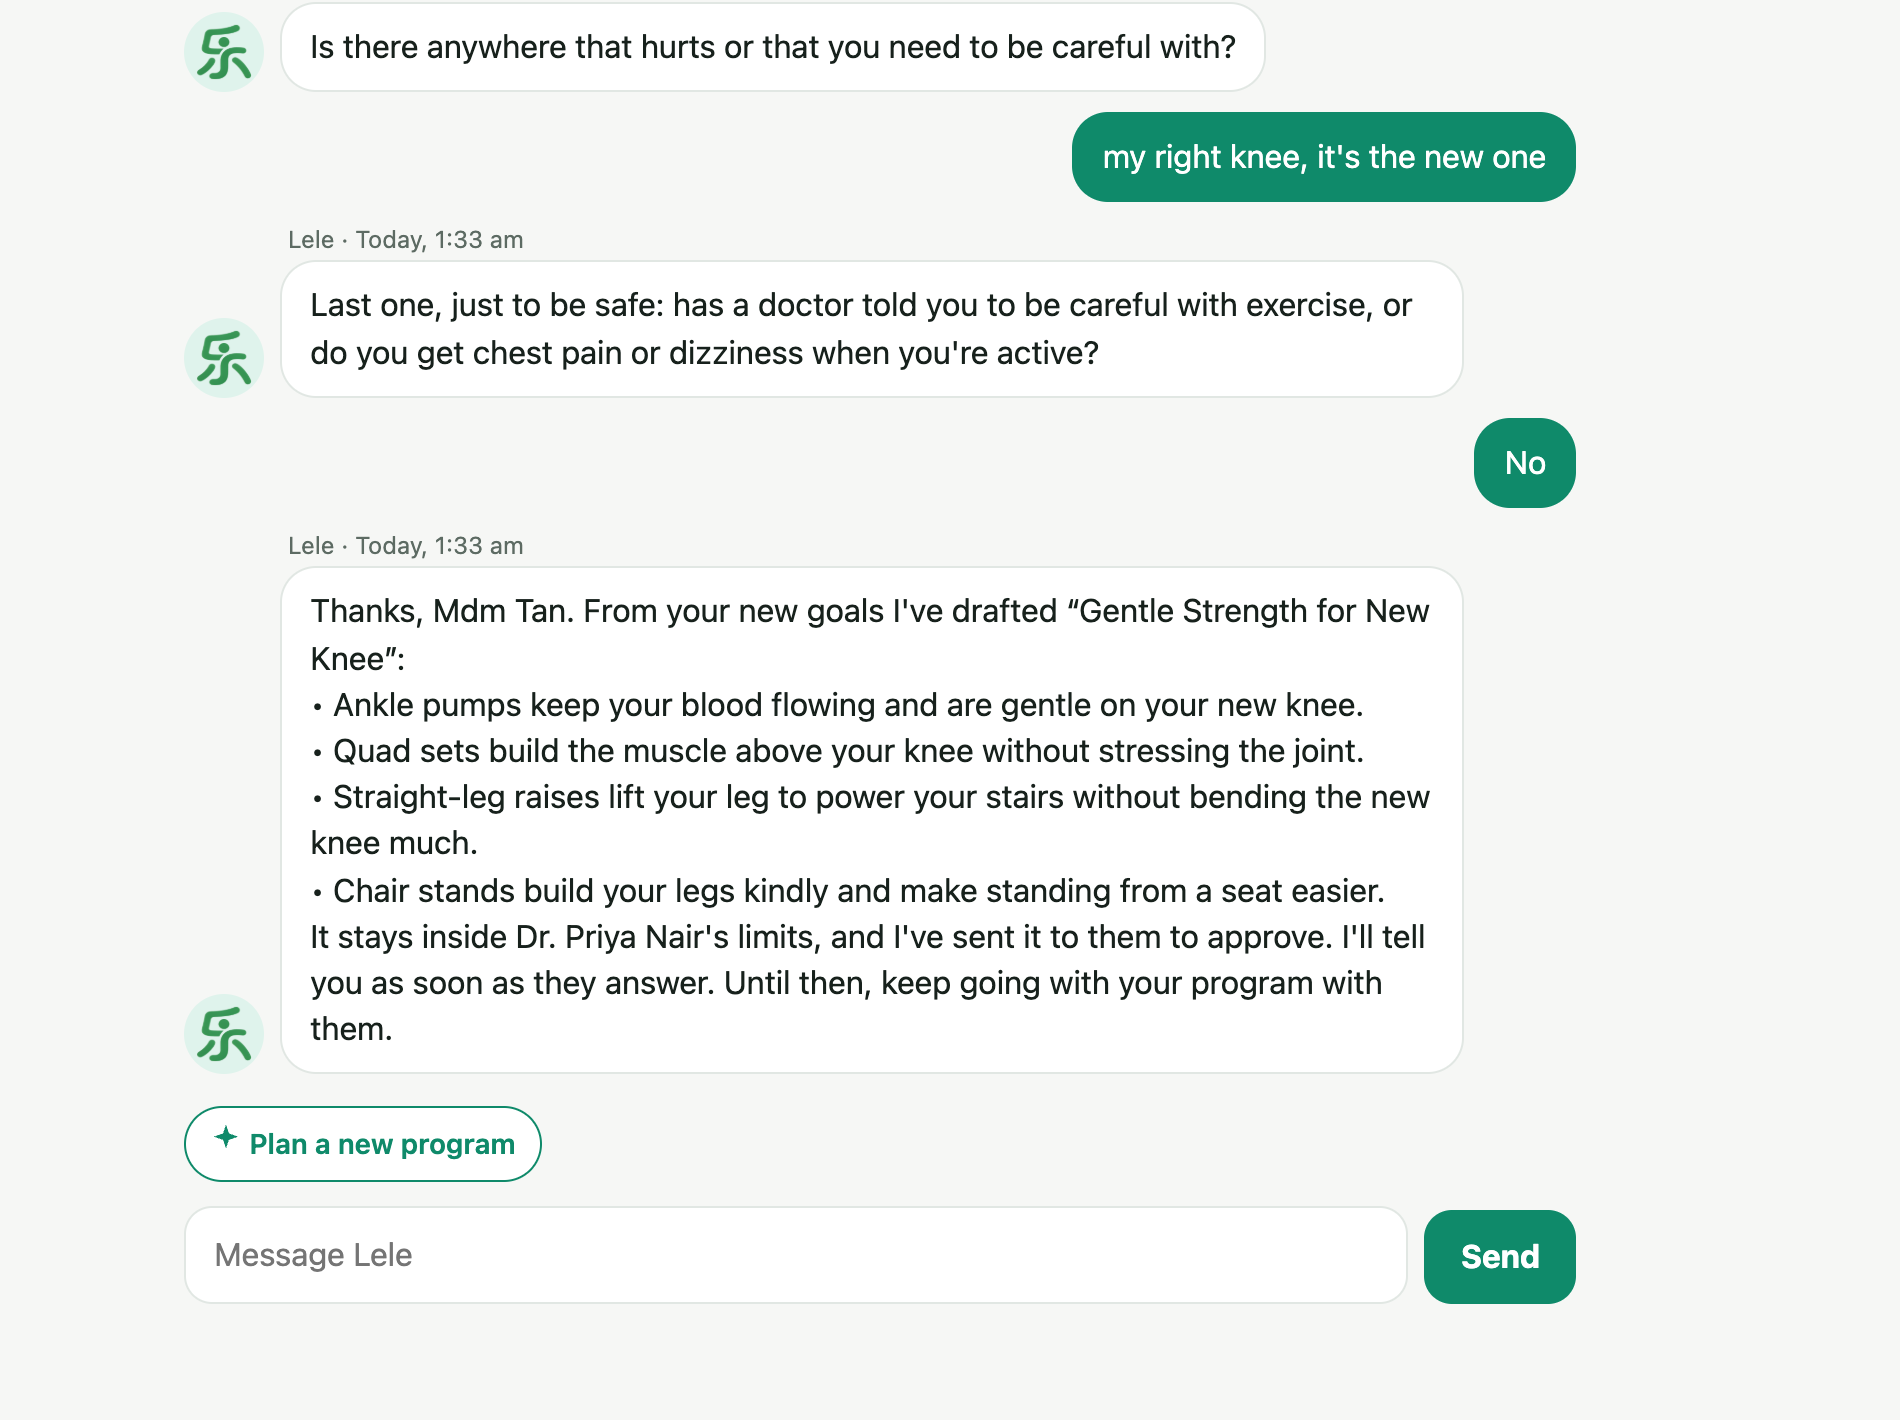
\includegraphics[width=\linewidth,height=0.78\textheight,keepaspectratio]{../screenshots/31-web-lele-plan-crop.png}}
\end{column}
\begin{column}{0.47\textwidth}
\begin{itemize}
  \item Tap \emph{Plan a new program}, or just say ``my goals have changed''.
  \item Five questions: goals, minutes, experience, what hurts, a safety check. Tap an answer or use your own words.
  \item Lele on \textbf{Tencent Cloud ADP} drafts the program from the knowledge base, using only Laile's vetted exercises. Code checks it against the person's limits.
  \item \textbf{No physio:} it replaces Lele's old plan and starts with a check-in.
  \item \textbf{Physio patient:} it goes to the physio to approve. Nothing starts before a yes.
\end{itemize}
\end{column}
\end{columns}
\end{frame}

% ---- 6c. Lele's record and brief -------------------------------------------
\begin{frame}{Lele learns each person, and briefs the physio}
\begin{columns}[T]
\begin{column}{0.37\textwidth}\centering
  \fbox{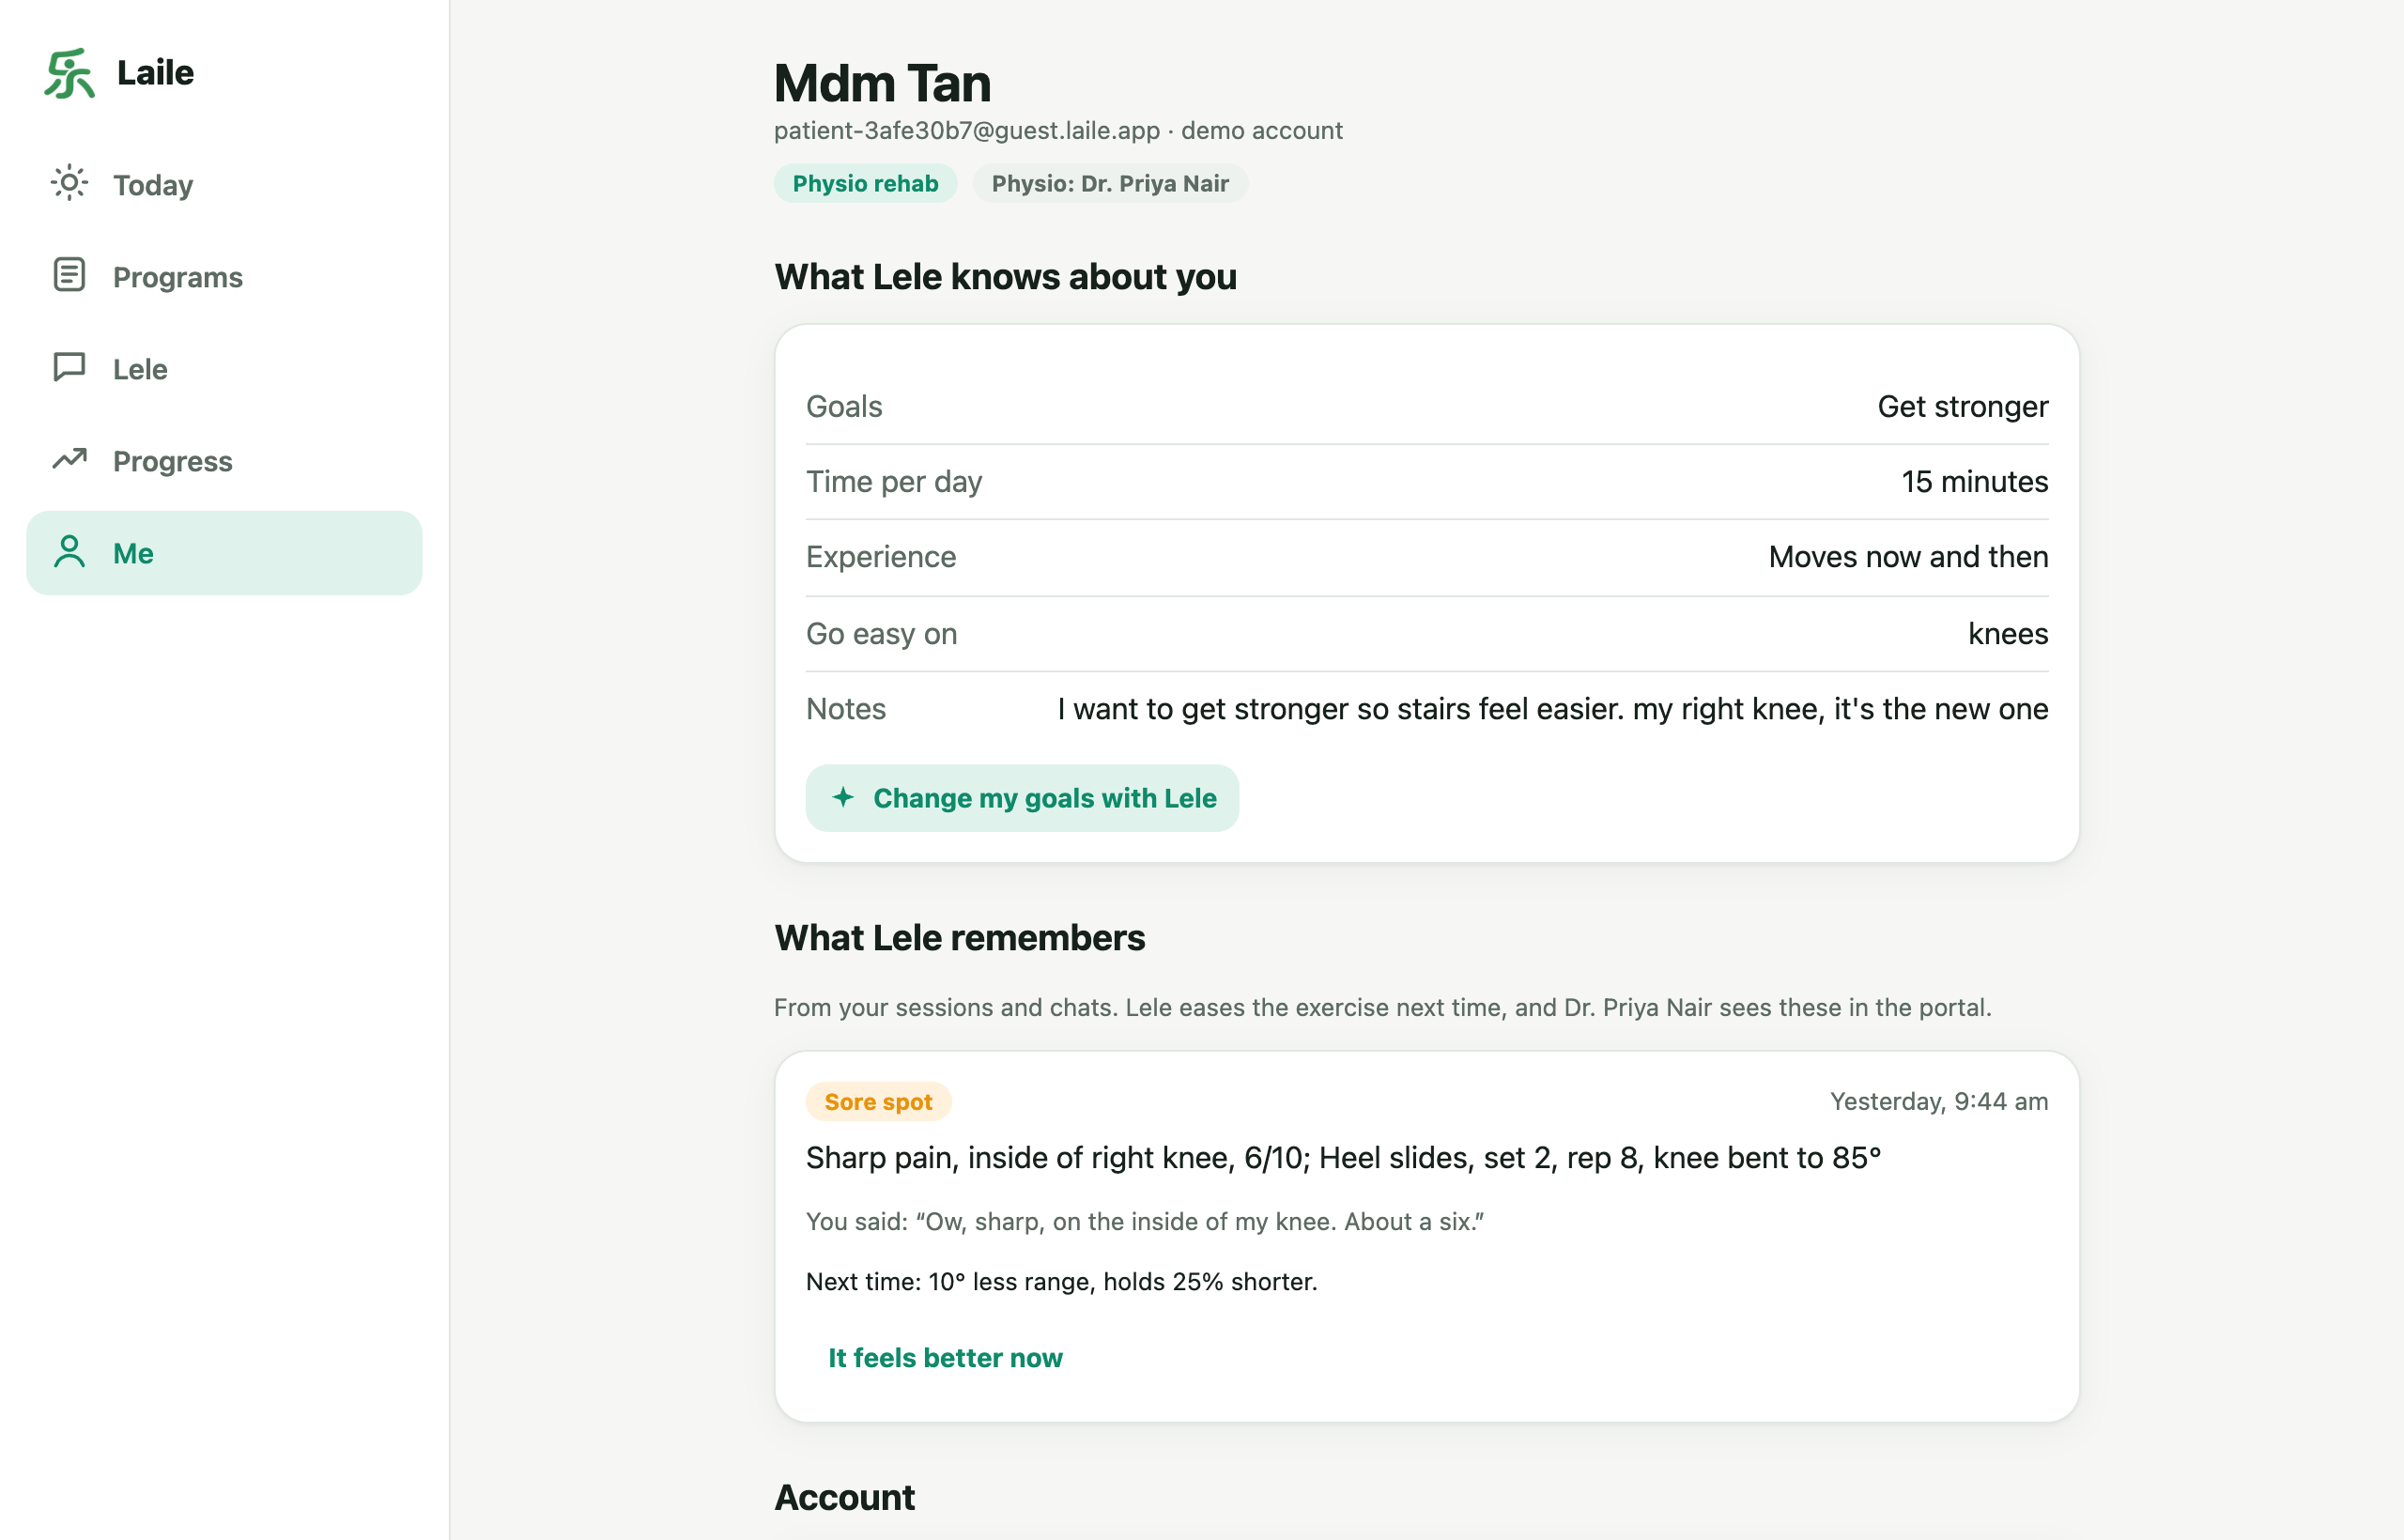
\includegraphics[width=\linewidth]{../screenshots/32-web-me.png}}\\[2pt]
  \capt{What Lele knows and remembers, on the person's Me screen}
\end{column}
\begin{column}{0.6\textwidth}\centering
  \fbox{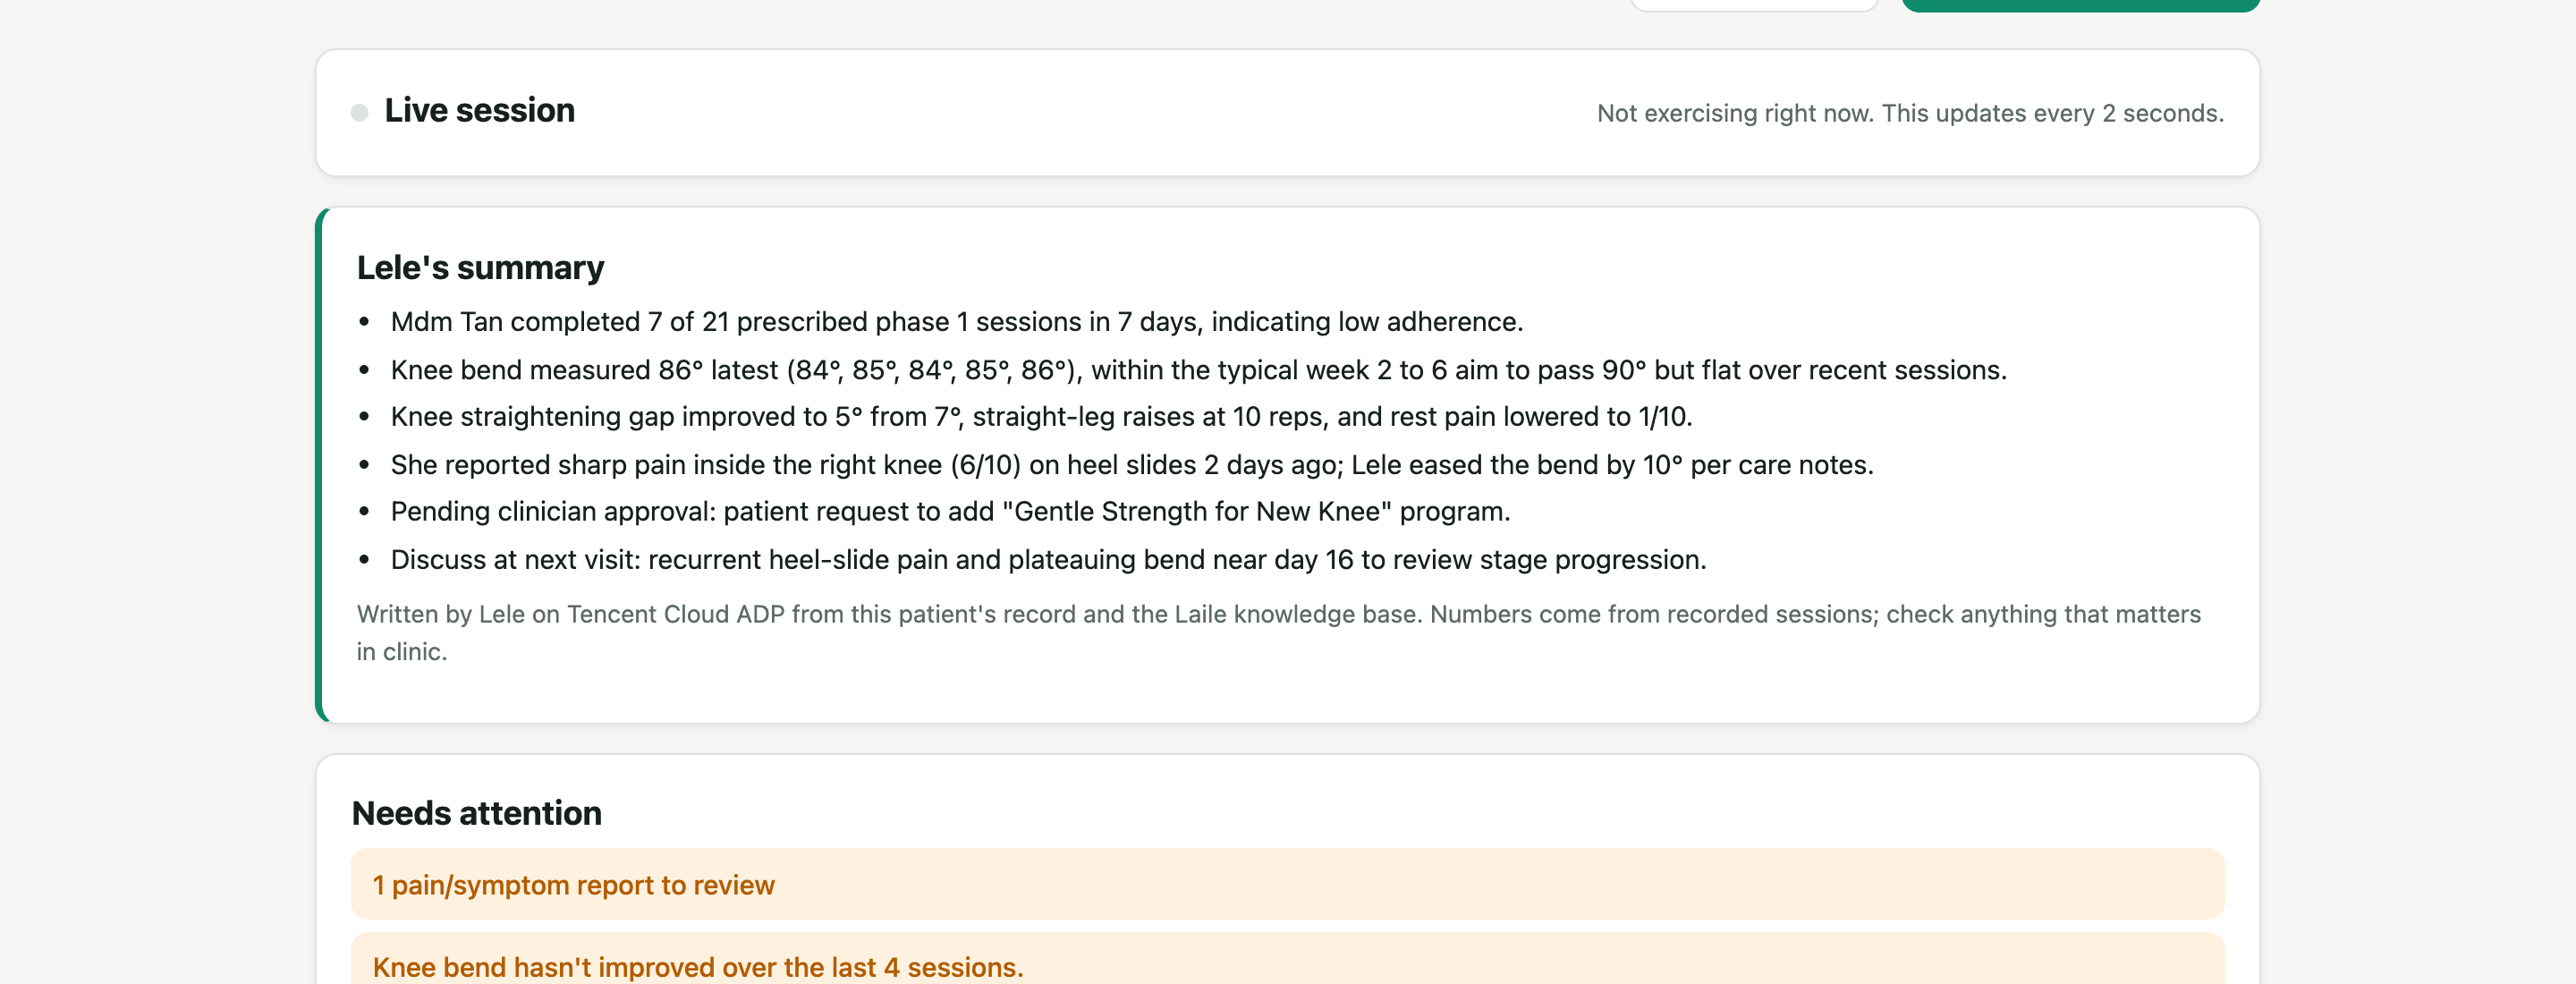
\includegraphics[width=\linewidth]{../screenshots/35-portal-patient-brief-crop.png}}\\[2pt]
  \capt{Lele's summary on the physio's patient page}
\end{column}
\end{columns}
\vspace{6pt}
\begin{itemize}
  \item Every chat and session adds to one record: goals, time, sore spots in their words, what was eased, measurements, requests.
  \item Lele reads it before every reply. For the physio, ADP writes a 4 to 6 line brief from that record plus the knowledge base (``typical week 2 to 6 aim to pass 90\textdegree''). The numbers come from code.
\end{itemize}
\end{frame}

% ---- 6d. Web --------------------------------------------------------------
\begin{frame}{Laile in any browser, no install}
\begin{columns}[T]
\begin{column}{0.7\textwidth}
  \fbox{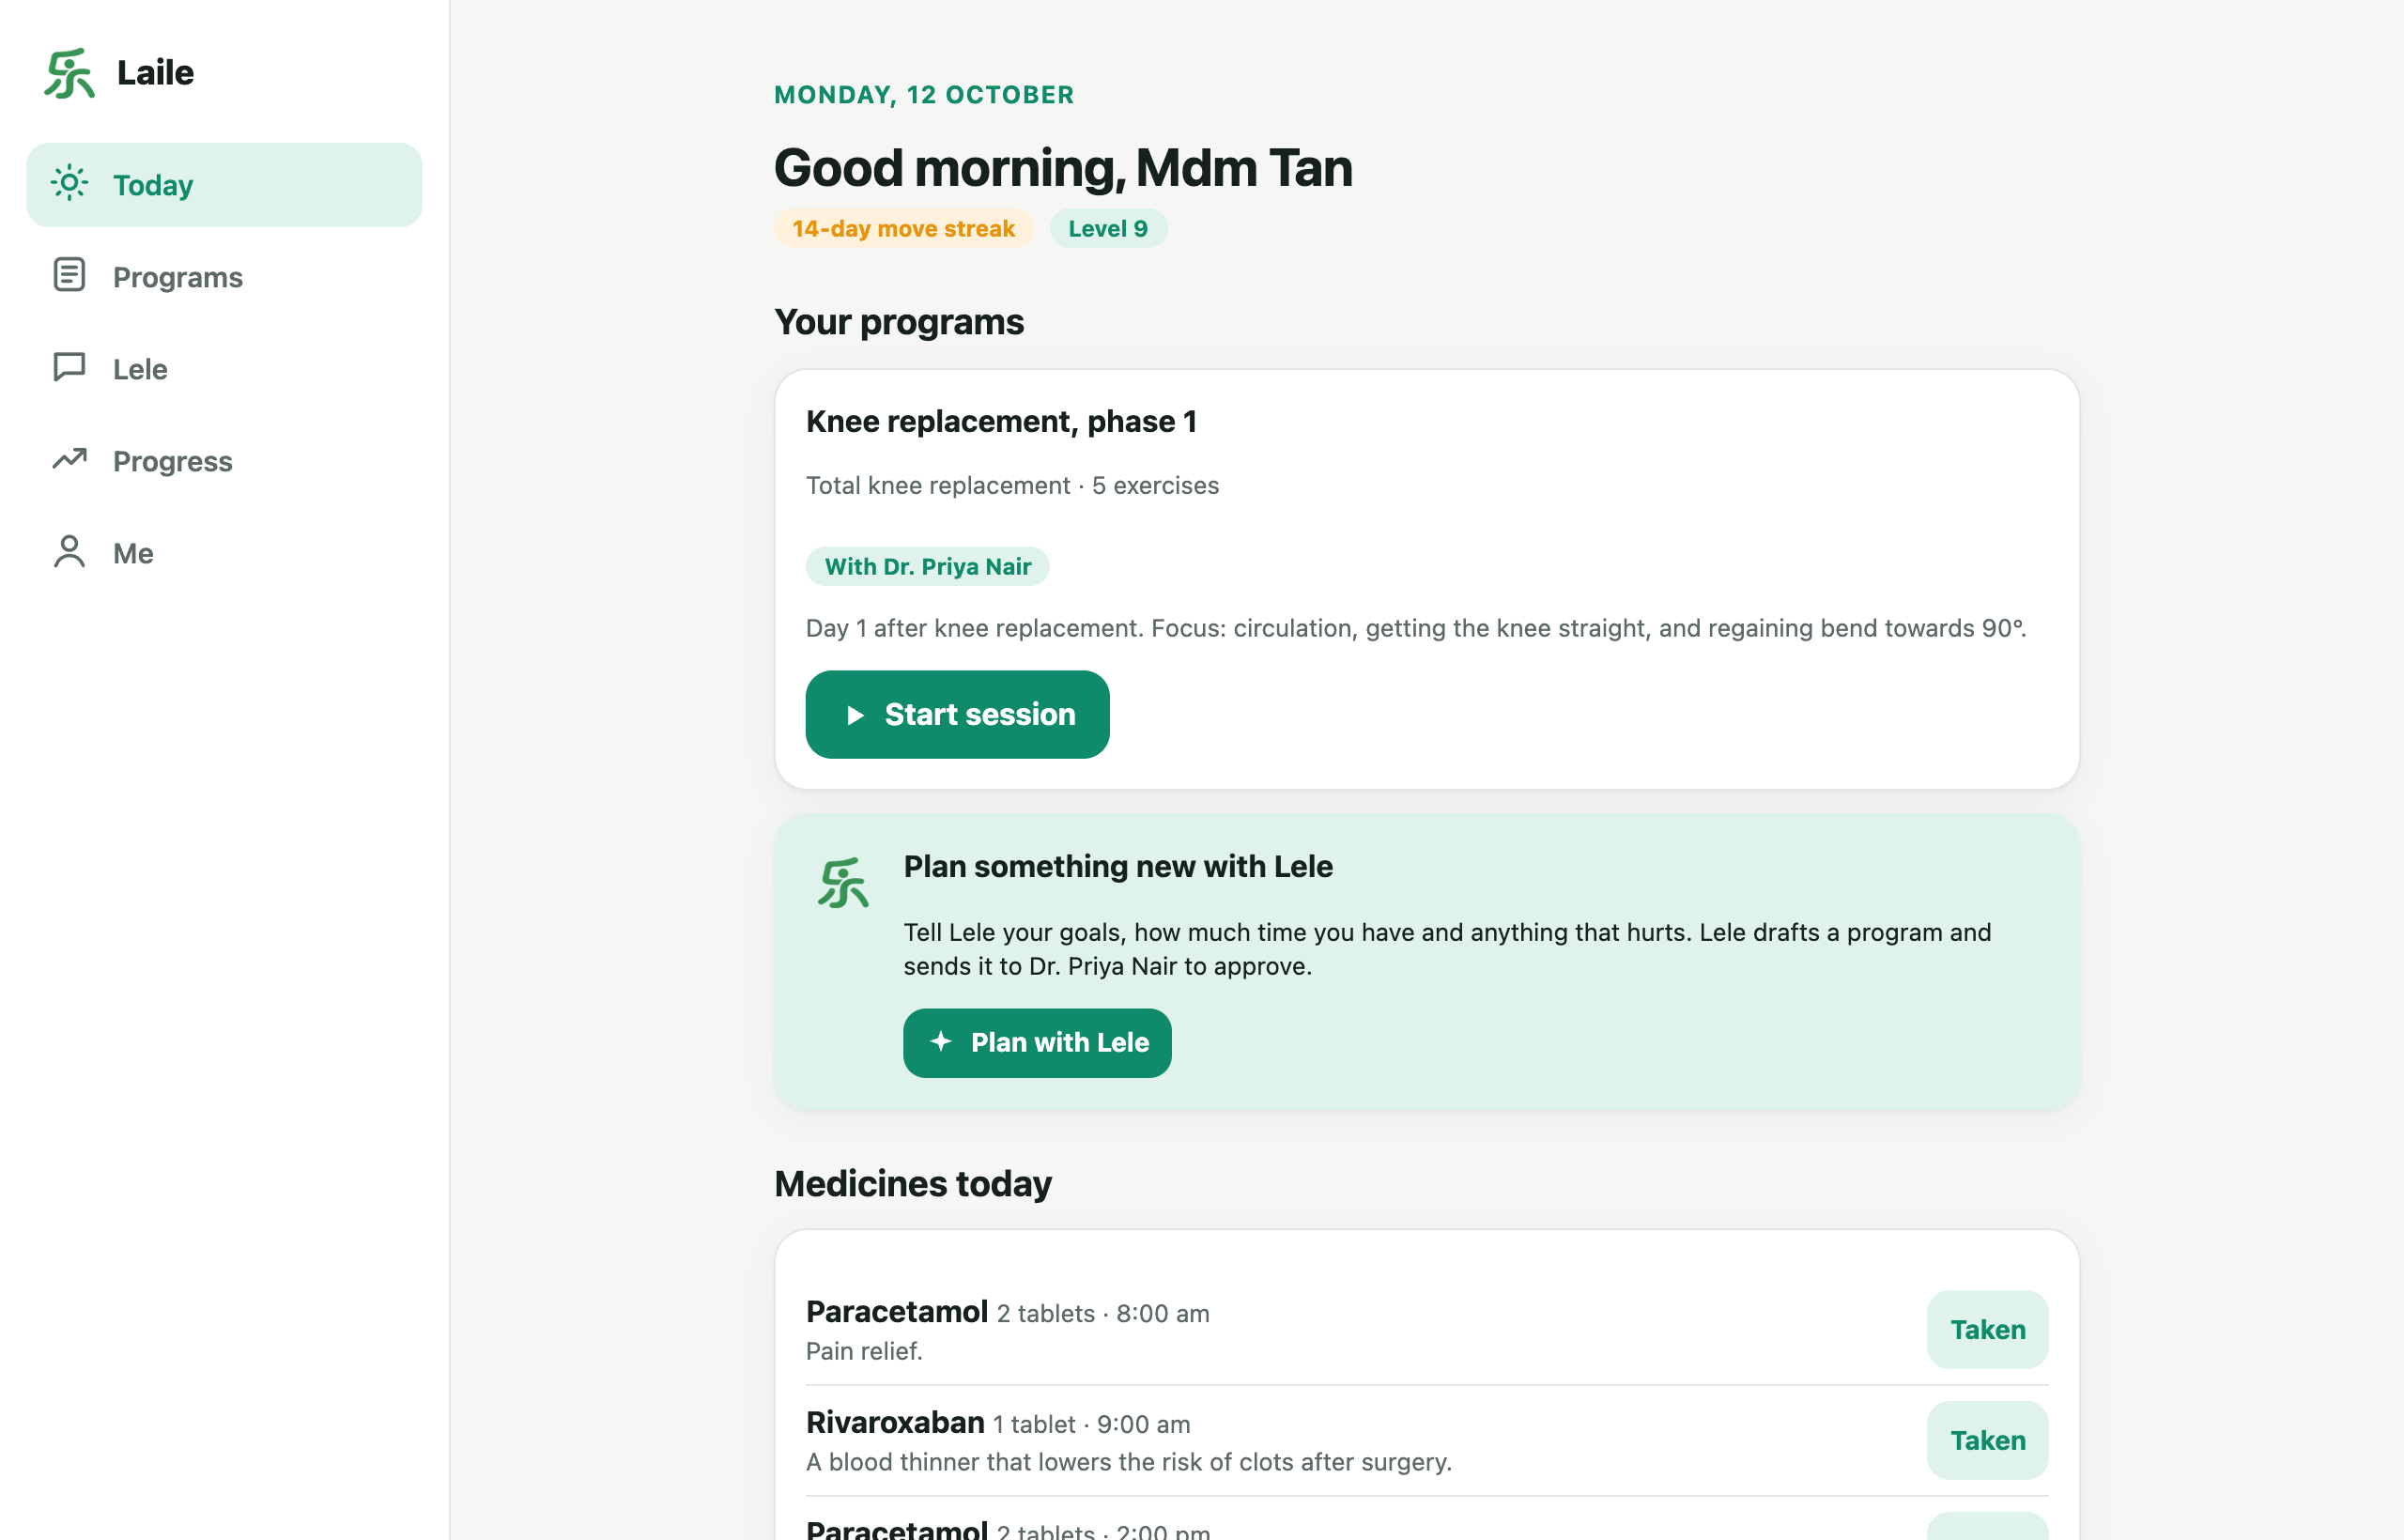
\includegraphics[width=0.47\linewidth]{../screenshots/30-web-today.png}}\hfill
  \fbox{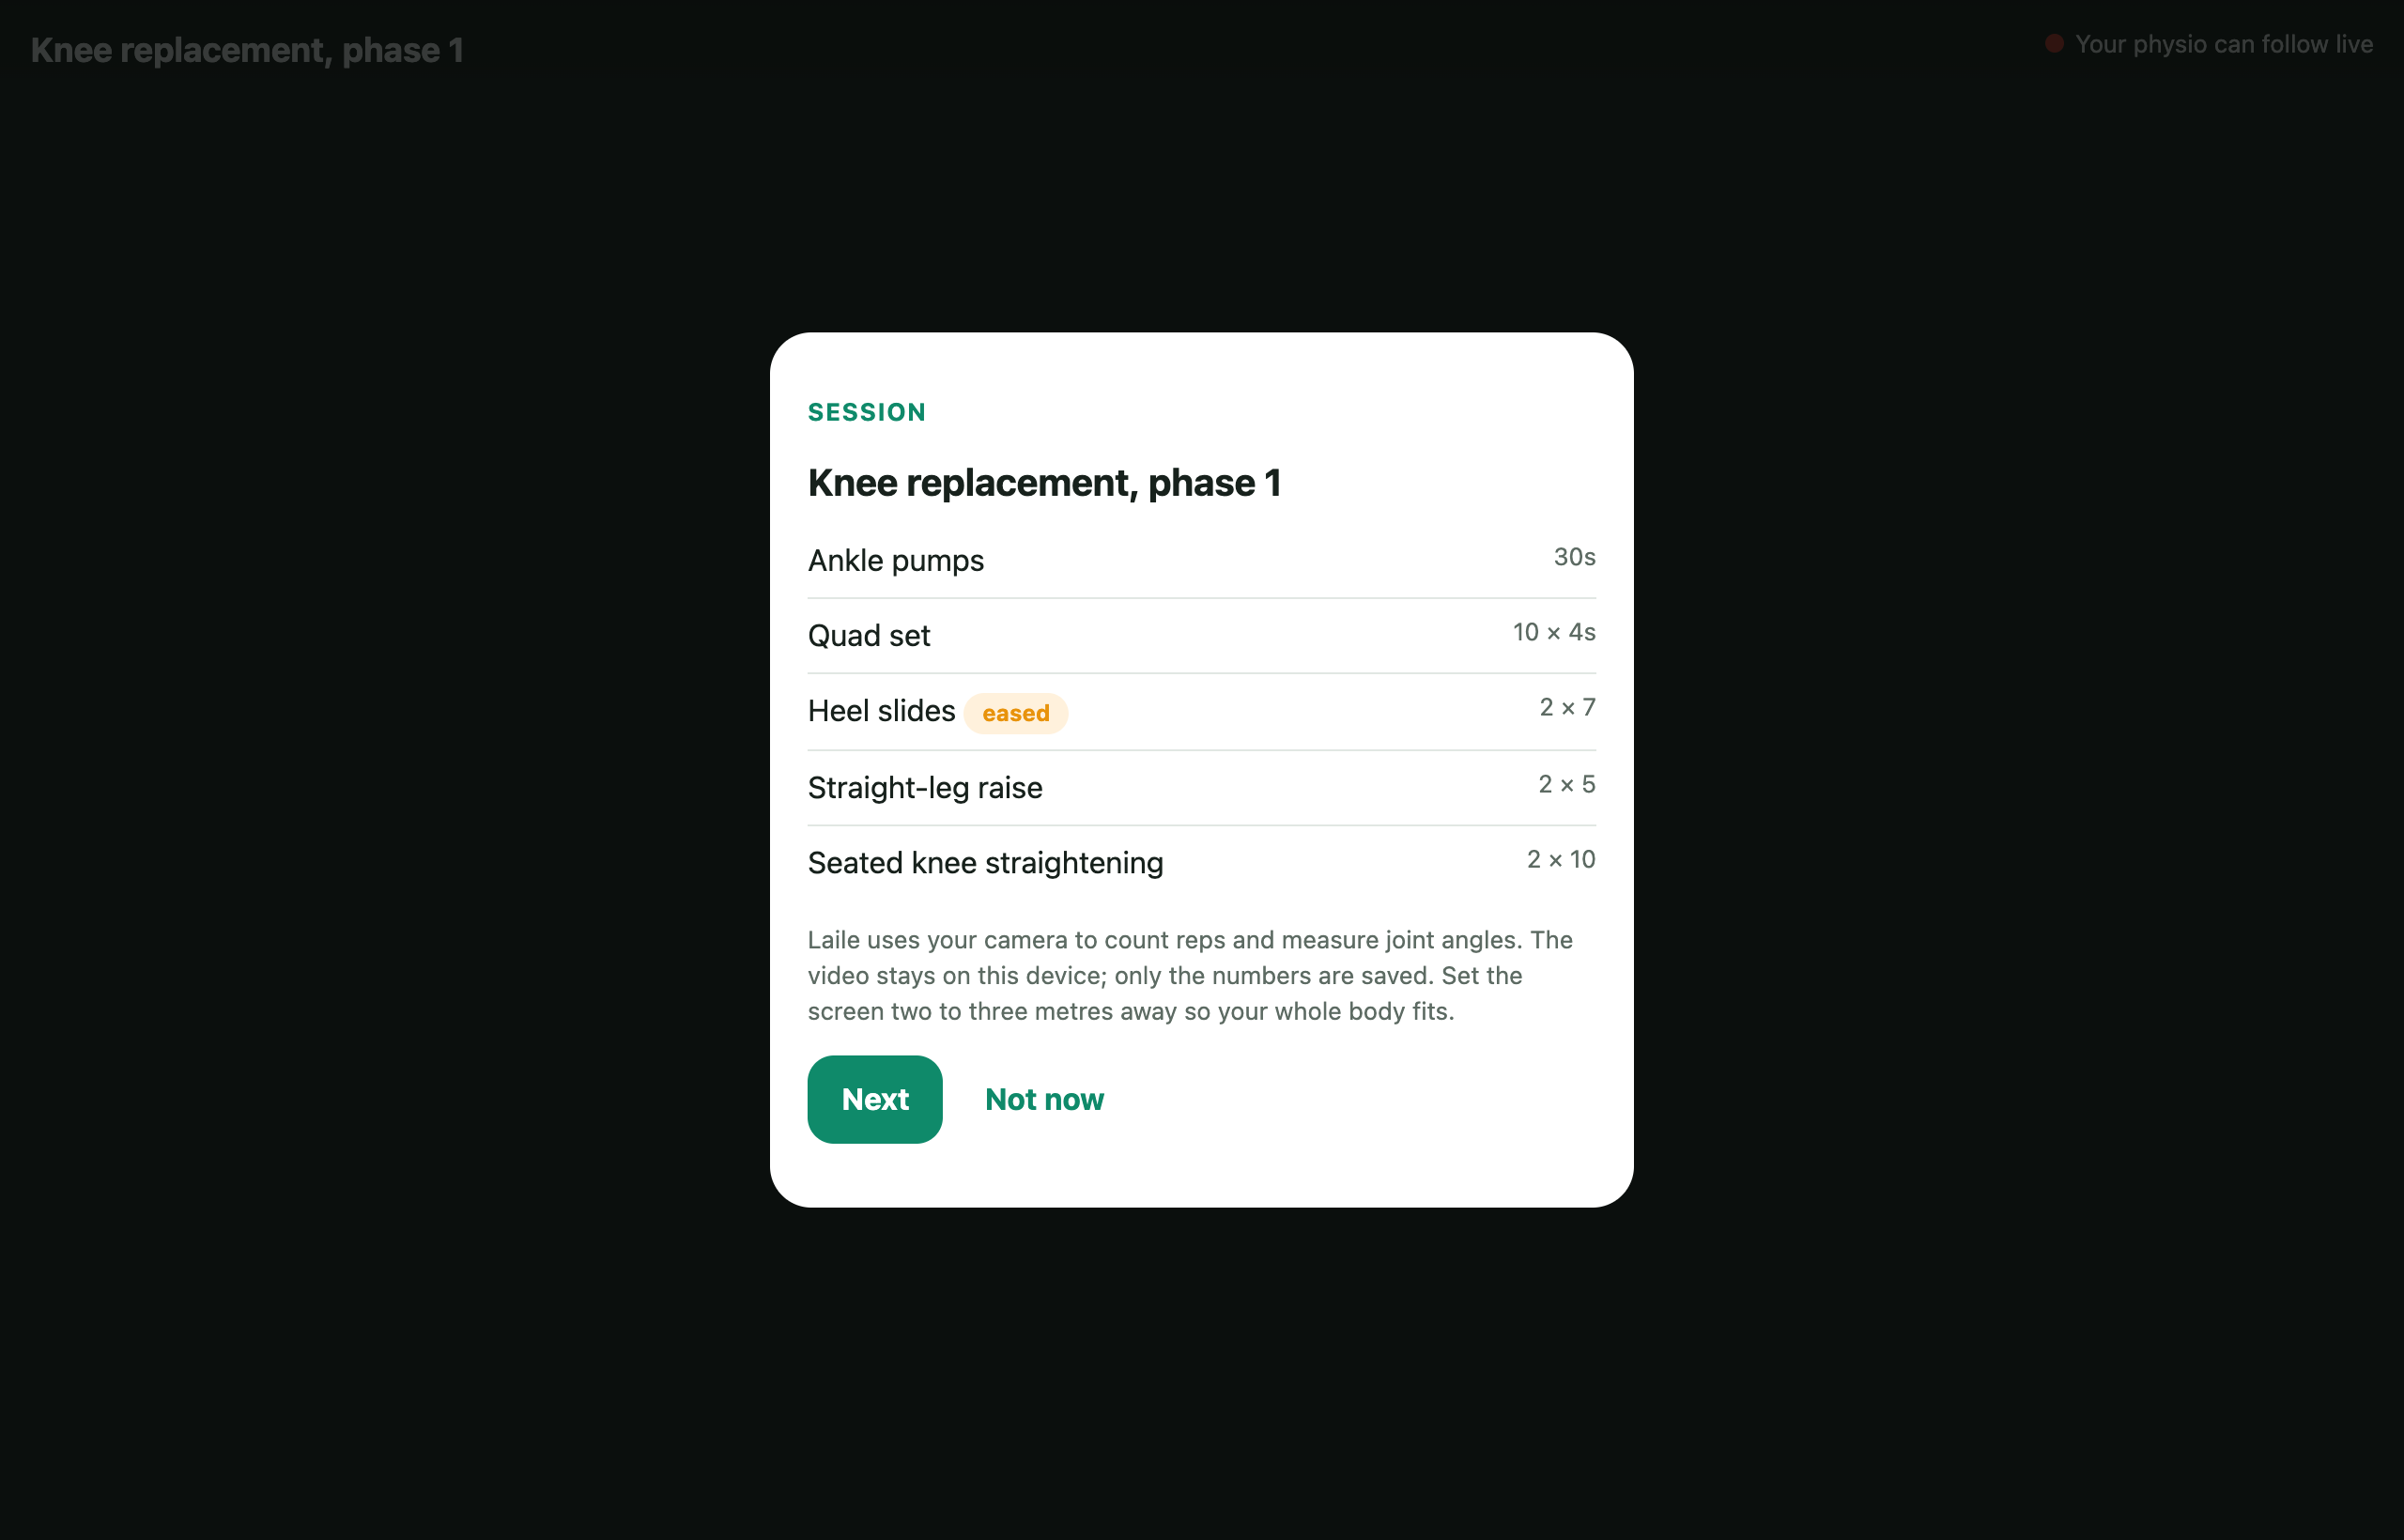
\includegraphics[width=0.47\linewidth]{../screenshots/33-web-session.png}}\\[2pt]
  \begin{minipage}[t]{0.47\linewidth}\centering\capt{Today on a laptop}\end{minipage}\hfill
  \begin{minipage}[t]{0.47\linewidth}\centering\capt{A webcam session; heel slides eased by Lele}\end{minipage}
  \begin{itemize}
    \item Same account, programs, Lele and progress as the iPhone app.
    \item MediaPipe pose in the browser and a port of Laile's session engine, tested against the same plan: web sessions count and report like phone sessions.
    \item Lele's ElevenLabs voice; the physio can watch live.
  \end{itemize}
\end{column}
\begin{column}{0.26\textwidth}\centering
  \fbox{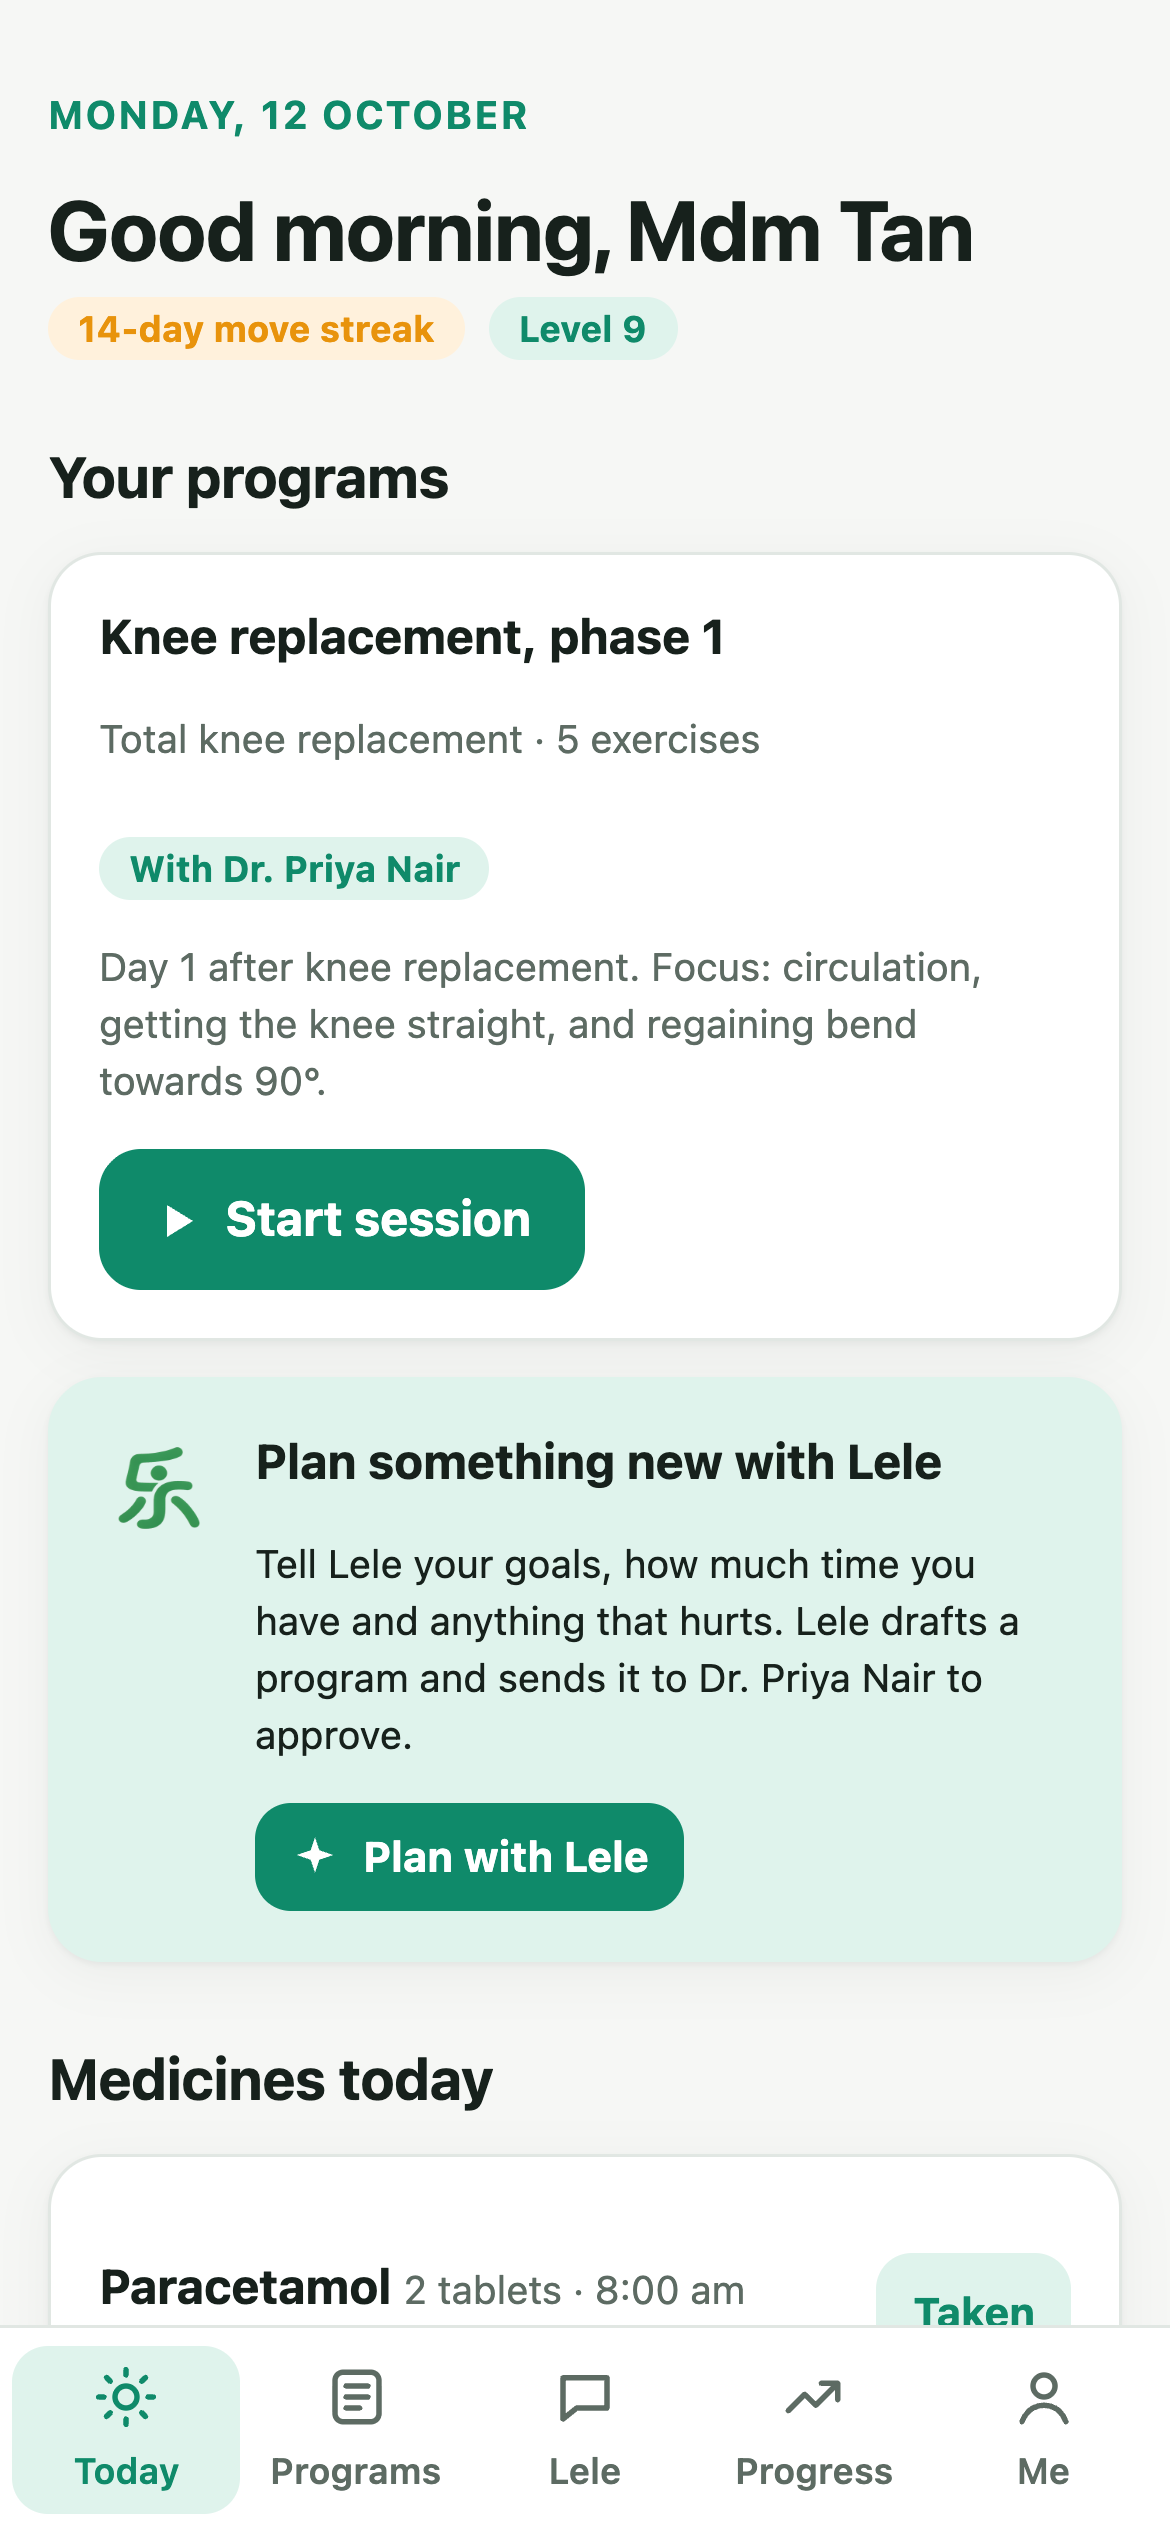
\includegraphics[height=0.64\textheight]{../screenshots/34-web-today-phone.png}}\\[2pt]
  \capt{43-156-108-79.sslip.io/app}
\end{column}
\end{columns}
\end{frame}

% ---- 7. Physio -----------------------------------------------------------
\begin{frame}{The physio stays on top}
\begin{columns}[c]
\begin{column}{0.62\textwidth}
  \fbox{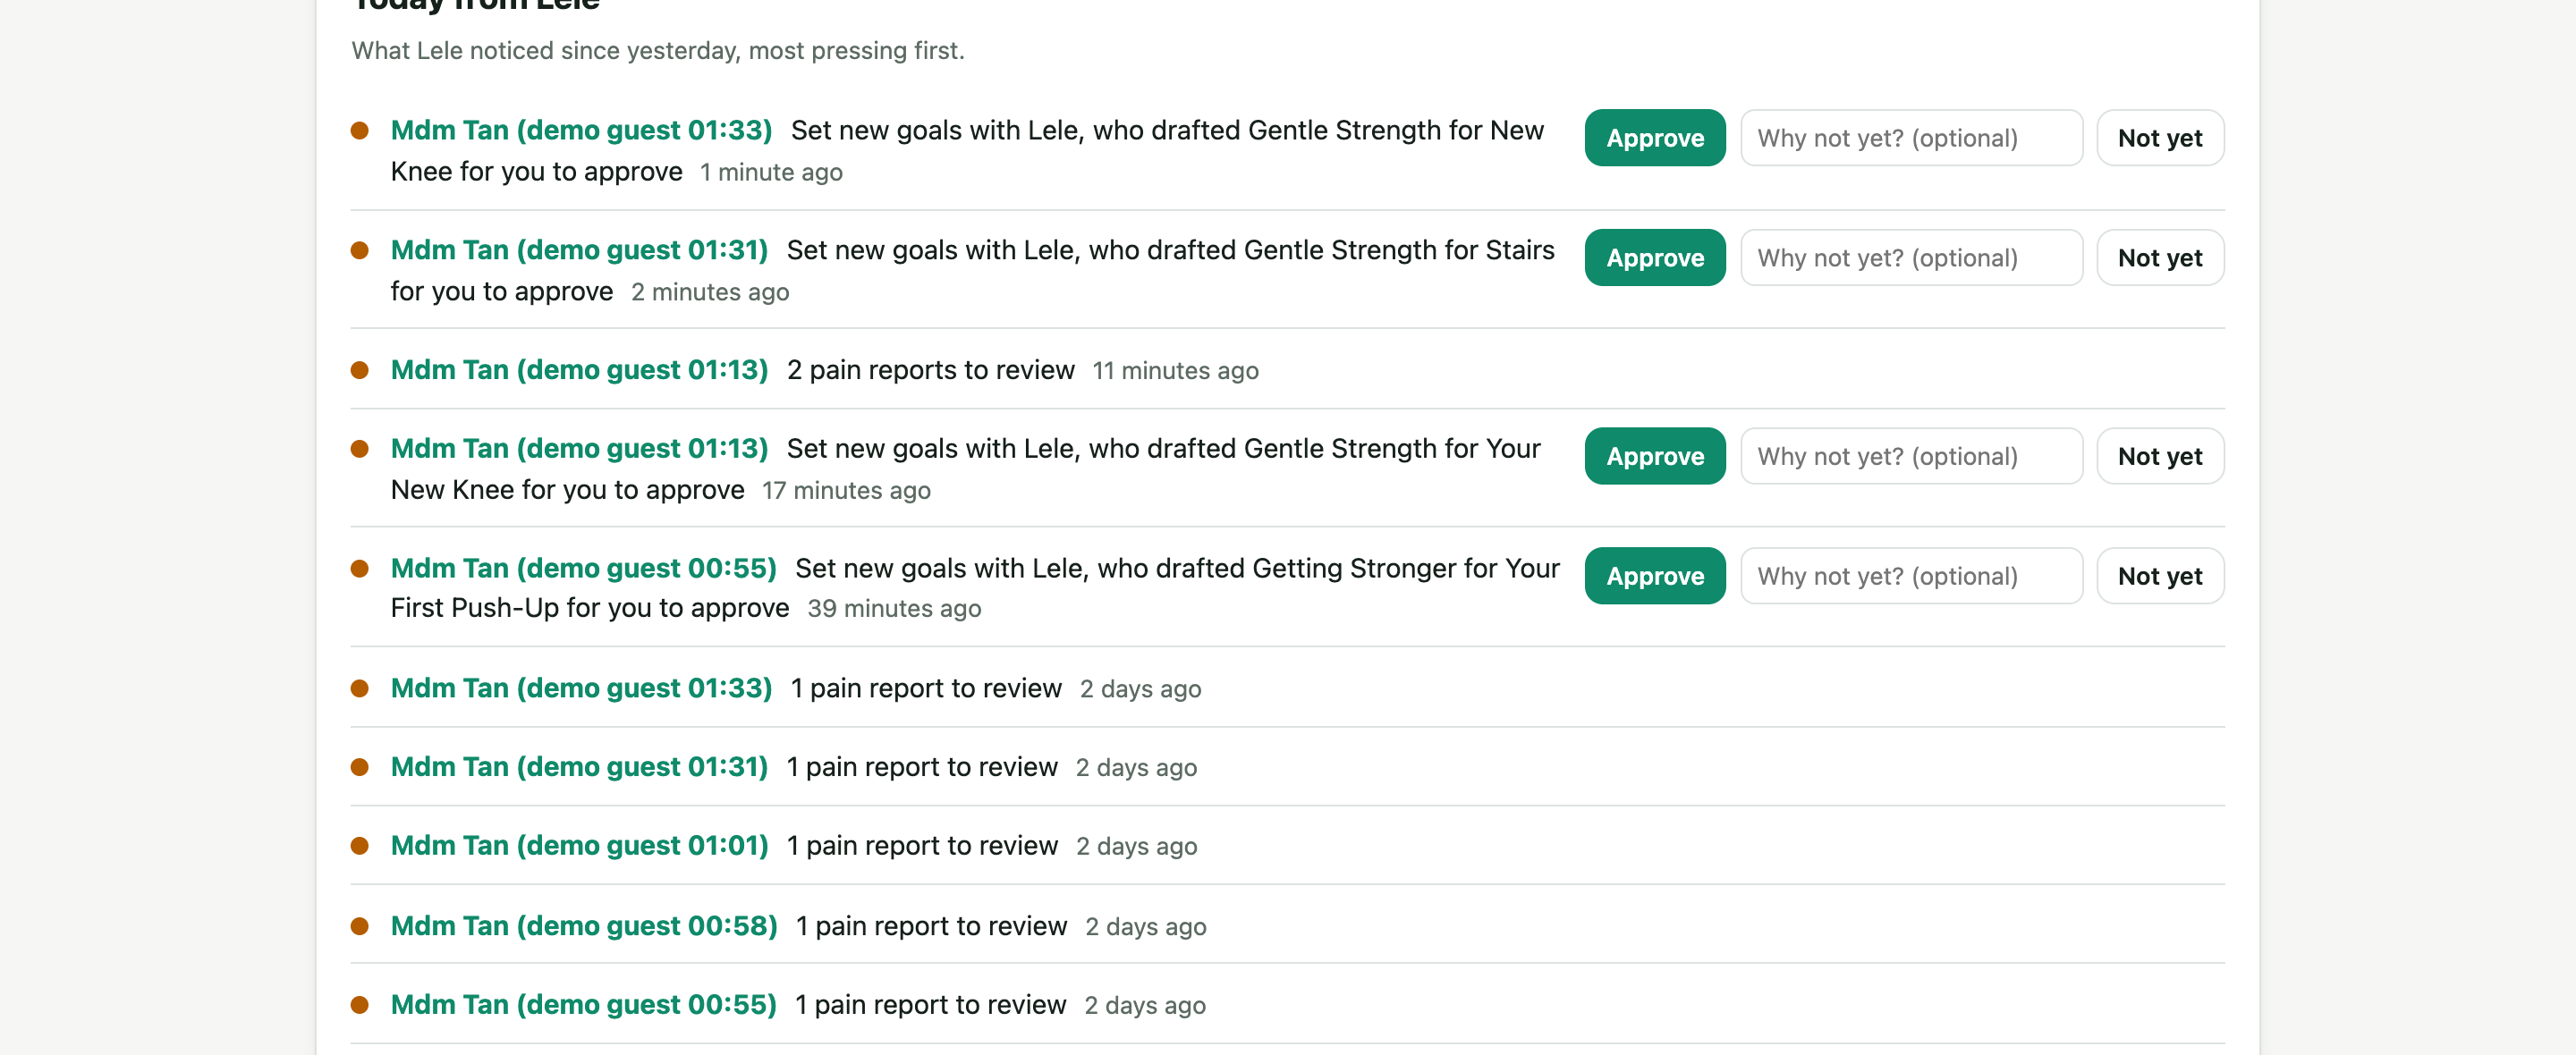
\includegraphics[width=\linewidth,height=0.7\textheight,keepaspectratio]{../screenshots/36-portal-lele-plan-approval-crop.png}}
\end{column}
\begin{column}{0.35\textwidth}
\begin{itemize}
  \item \textbf{Today from Lele}, most pressing first: red flags, worse this morning, pain reports, requests, missed days.
  \item \textbf{Live view} of a session: exercise, reps, measured angle.
  \item \textbf{Approve} extra programs and \textbf{Lele's plans}; \textbf{ask Lele} to change one in plain words; \textbf{sign} every version.
  \item \textbf{Discharge} hands the patient to a follow-on program, limits kept.
\end{itemize}
\end{column}
\end{columns}
\end{frame}

% ---- 8. Architecture ----------------------------------------------------
\begin{frame}{Architecture and trust boundary}
\centering
\resizebox{0.98\linewidth}{!}{% Laile architecture and trust boundary. Included by architecture.tex, the write-up and the deck.
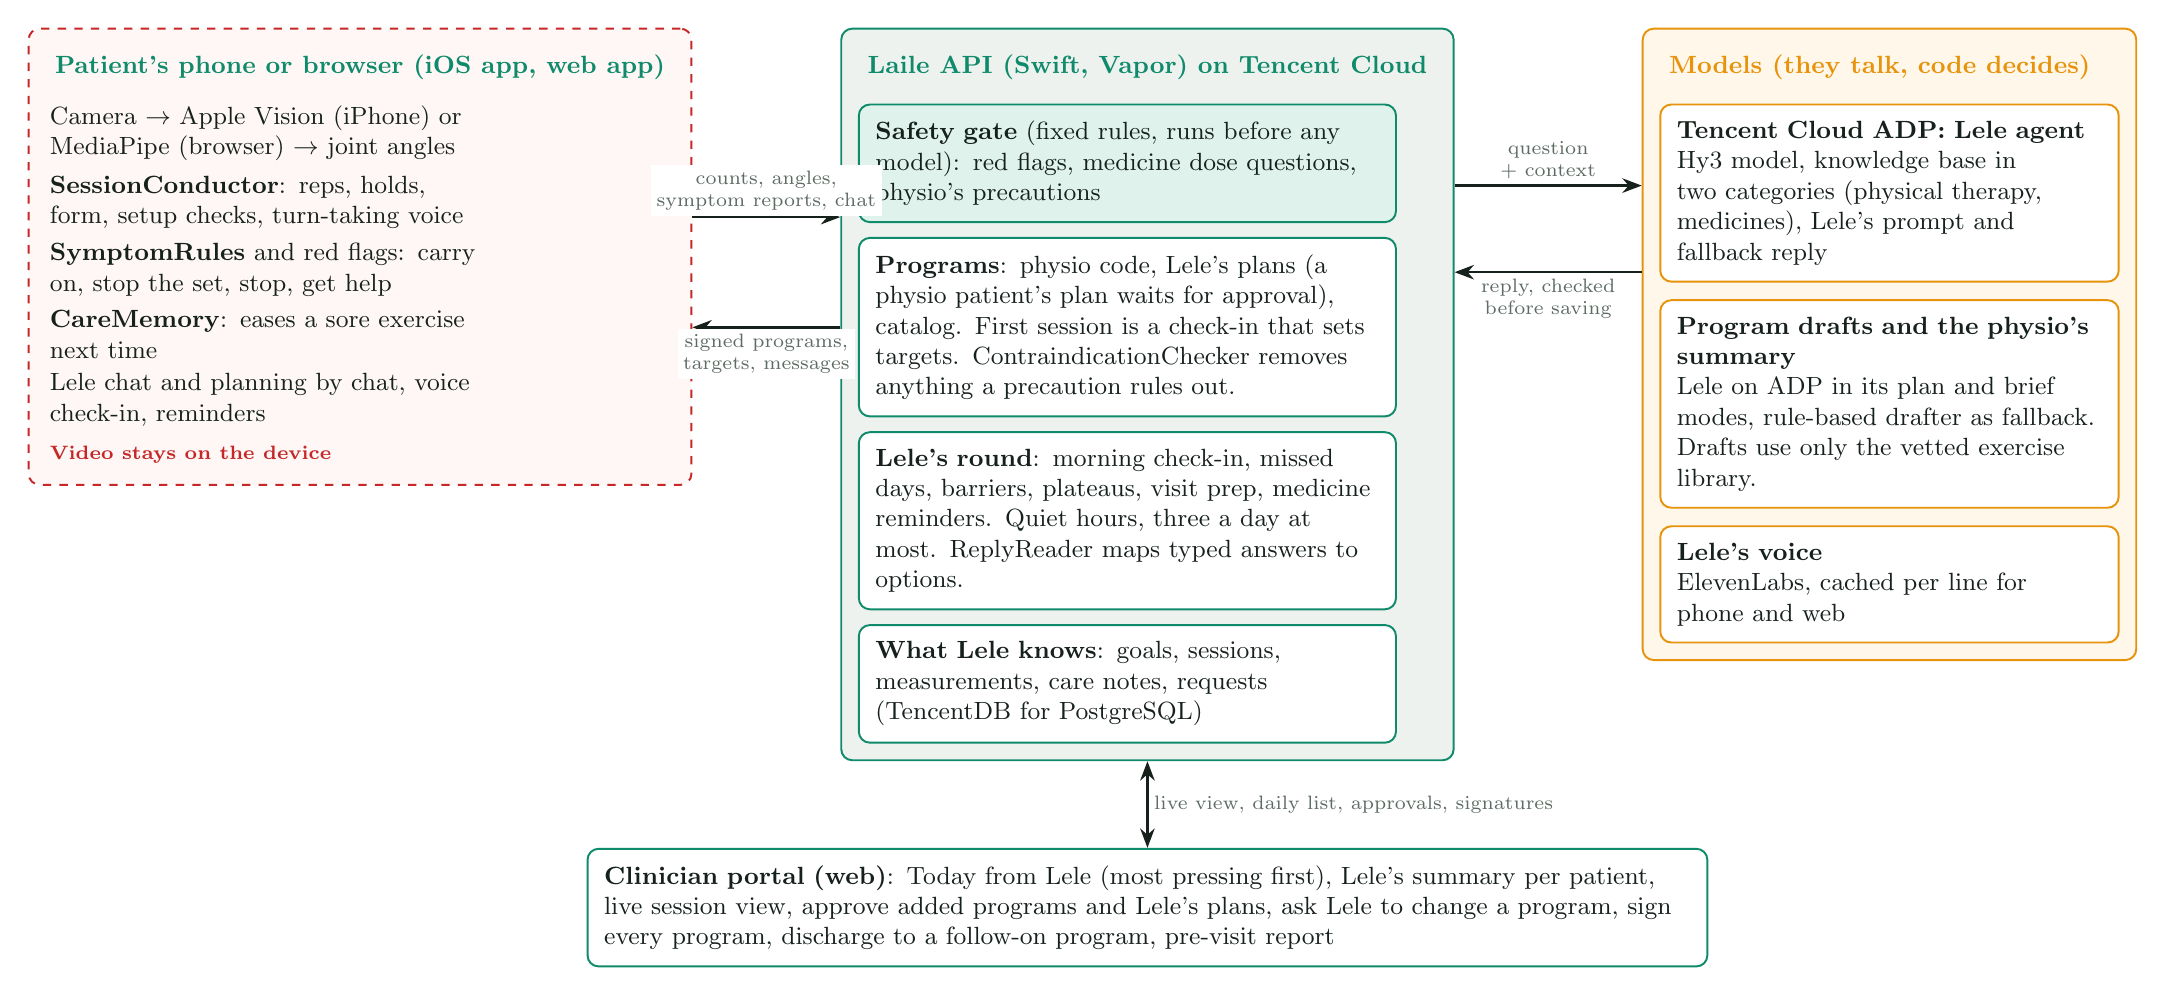
\begin{tikzpicture}[
    font=\small,
    every node/.style={text=ink, execute at begin node={\hyphenpenalty=10000\exhyphenpenalty=10000}},
    box/.style={draw=#1, fill=white, rounded corners=4pt, line width=0.7pt, align=left, inner sep=6pt},
    box/.default=accent,
    item/.style={align=left, text width=#1, inner sep=1.5pt},
    item/.default=5.6cm,
    title/.style={font=\small\bfseries, align=left},
    flow/.style={-{Stealth[length=7pt]}, line width=0.9pt, draw=ink},
    lab/.style={font=\scriptsize, text=muted, fill=white, inner sep=2pt, align=center},
  ]

  % --- Phone -------------------------------------------------------------
  \node[title, text=accent] (phoneT) at (0,0) {Patient's phone or browser (iOS app, web app)};
  \node[item, below=4pt of phoneT.south west, anchor=north west] (p1) {Camera $\rightarrow$ Apple Vision (iPhone) or MediaPipe (browser) $\rightarrow$ joint angles};
  \node[item, below=2pt of p1.south west, anchor=north west] (p2) {\textbf{SessionConductor}: reps, holds, form, setup checks, turn-taking voice};
  \node[item, below=2pt of p2.south west, anchor=north west] (p3) {\textbf{SymptomRules} and red flags: carry on, stop the set, stop, get help};
  \node[item, below=2pt of p3.south west, anchor=north west] (p4) {\textbf{CareMemory}: eases a sore exercise next time};
  \node[item, below=2pt of p4.south west, anchor=north west] (p5) {Lele chat and planning by chat, voice check-in, reminders};
  \node[item, below=4pt of p5.south west, anchor=north west, text=danger, font=\scriptsize\bfseries] (p6) {Video stays on the device};
  \begin{scope}[on background layer]
    \node[box=danger, dashed, fit=(phoneT)(p1)(p2)(p3)(p4)(p5)(p6), fill=dangersoft!35] (phone) {};
  \end{scope}

  % --- Laile API -----------------------------------------------------------
  \node[title, text=accent] (apiT) at (10.0,0) {Laile API (Swift, Vapor) on Tencent Cloud};
  \node[box, fill=accentsoft, below=5pt of apiT.south west, anchor=north west, text width=6.4cm] (gate)
    {\textbf{Safety gate} (fixed rules, runs before any model): red flags, medicine dose questions, physio's precautions};
  \node[box, below=5pt of gate, text width=6.4cm] (prog)
    {\textbf{Programs}: physio code, Lele's plans (a physio patient's plan waits for approval), catalog. First session is a check-in that sets targets. ContraindicationChecker removes anything a precaution rules out.};
  \node[box, below=5pt of prog, text width=6.4cm] (round)
    {\textbf{Lele's round}: morning check-in, missed days, barriers, plateaus, visit prep, medicine reminders. Quiet hours, three a day at most. ReplyReader maps typed answers to options.};
  \node[box, below=5pt of round, text width=6.4cm] (data)
    {\textbf{What Lele knows}: goals, sessions, measurements, care notes, requests (TencentDB for PostgreSQL)};
  \begin{scope}[on background layer]
    \node[box, fit=(apiT)(gate)(prog)(round)(data), fill=surface] (api) {};
  \end{scope}

  % --- AI services ---------------------------------------------------------
  \node[title, text=reward] (aiT) at (19.3,0) {Models (they talk, code decides)};
  \node[box=reward, below=5pt of aiT.south west, anchor=north west, text width=5.4cm] (adp)
    {\textbf{Tencent Cloud ADP: Lele agent}\\ Hy3 model, knowledge base in two categories (physical therapy, medicines), Lele's prompt and fallback reply};
  \node[box=reward, below=6pt of adp, text width=5.4cm] (hy)
    {\textbf{Program drafts and the physio's summary}\\ Lele on ADP in its plan and brief modes, rule-based drafter as fallback. Drafts use only the vetted exercise library.};
  \node[box=reward, below=6pt of hy, text width=5.4cm] (voice)
    {\textbf{Lele's voice}\\ ElevenLabs, cached per line for phone and web};
  \begin{scope}[on background layer]
    \node[box=reward, fit=(aiT)(adp)(hy)(voice), fill=rewardsoft!60] (ai) {};
  \end{scope}

  % --- Portal --------------------------------------------------------------
  \node[box, below=1.1cm of api, text width=13.8cm, xshift=0cm] (portal)
    {\textbf{Clinician portal (web)}: Today from Lele (most pressing first), Lele's summary per patient, live session view, approve added programs and Lele's plans, ask Lele to change a program, sign every program, discharge to a follow-on program, pre-visit report};

  % --- Flows (horizontal, at fixed heights) ------------------------------------
  \draw[flow] (phone.east |- 0,-1.9) -- node[lab, above, pos=0.5] {counts, angles,\\symptom reports, chat} (api.west |- 0,-1.9);
  \draw[flow] (api.west |- 0,-3.3) -- node[lab, below, pos=0.5] {signed programs,\\targets, messages} (phone.east |- 0,-3.3);
  \draw[flow] (api.east |- 0,-1.5) -- node[lab, above, pos=0.5] {question\\+ context} (ai.west |- 0,-1.5);
  \draw[flow] (ai.west |- 0,-2.6) -- node[lab, below, pos=0.5] {reply, checked\\before saving} (api.east |- 0,-2.6);
  \draw[flow, {Stealth[length=7pt]}-{Stealth[length=7pt]}] (api.south) -- node[lab, right] {live view, daily list, approvals, signatures} (portal.north -| api.south);
\end{tikzpicture}
}
\end{frame}

% ---- 9. AI and safety ---------------------------------------------------
\begin{frame}{How the AI is used, and kept safe}
\footnotesize
\begin{tabularx}{\linewidth}{@{}>{\raggedright\arraybackslash}p{3.3cm}>{\raggedright\arraybackslash}p{4.4cm}>{\raggedright\arraybackslash}X@{}}
\toprule
\textbf{Job} & \textbf{Done by} & \textbf{Kept safe by}\\
\midrule
Conversation and explanations & Lele on \textbf{Tencent Cloud ADP} (Hy3, 12-document knowledge base) & Real context sent with each message; red flags and dose questions answered by rules first\\
Remembering what hurt & Care notes & Easing computed by code; physio sees every note\\
Program drafts & Lele on \textbf{ADP} (plan mode, knowledge base); rule-based fallback & Vetted library only, precautions enforced, physio signs or approves\\
Brief for the physio & Lele on \textbf{ADP} (brief mode) with the record and knowledge base & Numbers and flags computed by code and passed in\\
Understanding replies & Keyword rules & ``Lele heard: \ldots''; asks again if unclear\\
Seeing movement & Apple Vision (iPhone), MediaPipe (browser) & Video stays on the device\\
\bottomrule
\end{tabularx}\\[8pt]
\begin{itemize}
  \item Dose questions: fixed referral to the doctor or pharmacist. Unknown medicine: \emph{``I'm not able to identify that medication, please check with your pharmacist.''}
  \item 166 automated tests cover counting, safety rules, care notes, Lele's round, planning by chat, the server flows and the web session engine.
\end{itemize}
\end{frame}

% ---- 9b. Stack ----------------------------------------------------------
\begin{frame}{Built with}
\vspace{4pt}
\centering
\resizebox{0.98\linewidth}{!}{% Laile's tech stack in three columns. Included by the write-up and the deck.
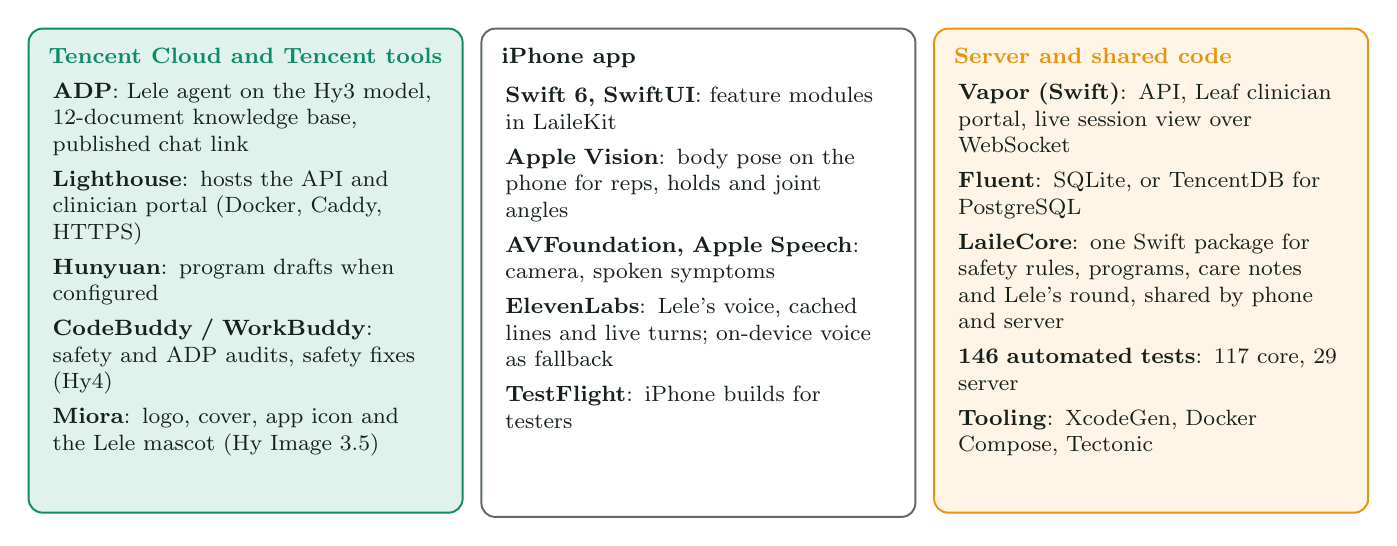
\begin{tikzpicture}[
    font=\fontsize{8}{9.6}\selectfont,
    every node/.style={text=ink, execute at begin node={\hyphenpenalty=10000\exhyphenpenalty=10000}},
    head/.style={font=\fontsize{8.5}{10}\selectfont\bfseries, text=#1, align=left, anchor=north west, inner sep=0pt},
    item/.style={align=left, anchor=north west, text width=4.9cm, inner sep=1.5pt},
    group/.style={draw=#1, rounded corners=5pt, line width=0.7pt, inner sep=7pt},
  ]
  \newcommand{\stackcol}[5]{%
    % #1 x, #2 name, #3 colour, #4 title, #5 items
    \node[head=#3] (#2-t) at (#1,0) {#4};
    \node[item, below=5pt of #2-t.south west, anchor=north west] (#2-b) {\parbox[t][5.15cm][t]{4.9cm}{#5}};
  }

  \stackcol{0}{tc}{accent}{Tencent Cloud and Tencent tools}{%
    \textbf{ADP}: Lele agent on the Hy3 model, 12-document knowledge base, published chat link\\[3pt]
    \textbf{Lighthouse}: hosts the API and clinician portal (Docker, Caddy, HTTPS)\\[3pt]
    \textbf{Hunyuan}: program drafts when configured\\[3pt]
    \textbf{CodeBuddy / WorkBuddy}: safety and ADP audits, safety fixes (Hy4)\\[3pt]
    \textbf{Miora}: logo, cover, app icon and the Lele mascot (Hy Image 3.5)}

  \stackcol{5.75}{ph}{ink}{iPhone app}{%
    \textbf{Swift 6, SwiftUI}: feature modules in LaileKit\\[3pt]
    \textbf{Apple Vision}: body pose on the phone for reps, holds and joint angles\\[3pt]
    \textbf{AVFoundation, Apple Speech}: camera, spoken symptoms\\[3pt]
    \textbf{ElevenLabs}: Lele's voice, cached lines and live turns; on-device voice as fallback\\[3pt]
    \textbf{TestFlight}: iPhone builds for testers}

  \stackcol{11.5}{sv}{reward}{Server and shared code}{%
    \textbf{Vapor (Swift)}: API, Leaf clinician portal, live session view over WebSocket\\[3pt]
    \textbf{Fluent}: SQLite, or TencentDB for PostgreSQL\\[3pt]
    \textbf{LaileCore}: one Swift package for safety rules, programs, care notes and Lele's round, shared by phone and server\\[3pt]
    \textbf{146 automated tests}: 117 core, 29 server\\[3pt]
    \textbf{Tooling}: XcodeGen, Docker Compose, Tectonic}

  \begin{scope}[on background layer]
    \node[group=accent, fill=accentsoft, fit=(tc-t)(tc-b)] {};
    \node[group=muted, fill=white, fit=(ph-t)(ph-b)] {};
    \node[group=reward, fill=rewardsoft!70, fit=(sv-t)(sv-b)] {};
  \end{scope}
\end{tikzpicture}
}
\end{frame}

% ---- 9c. Tencent tools in the build --------------------------------------
\begin{frame}{Made with Tencent's own tools}
\small
\begin{columns}[T]
\begin{column}{0.36\textwidth}
  \centering
  \fbox{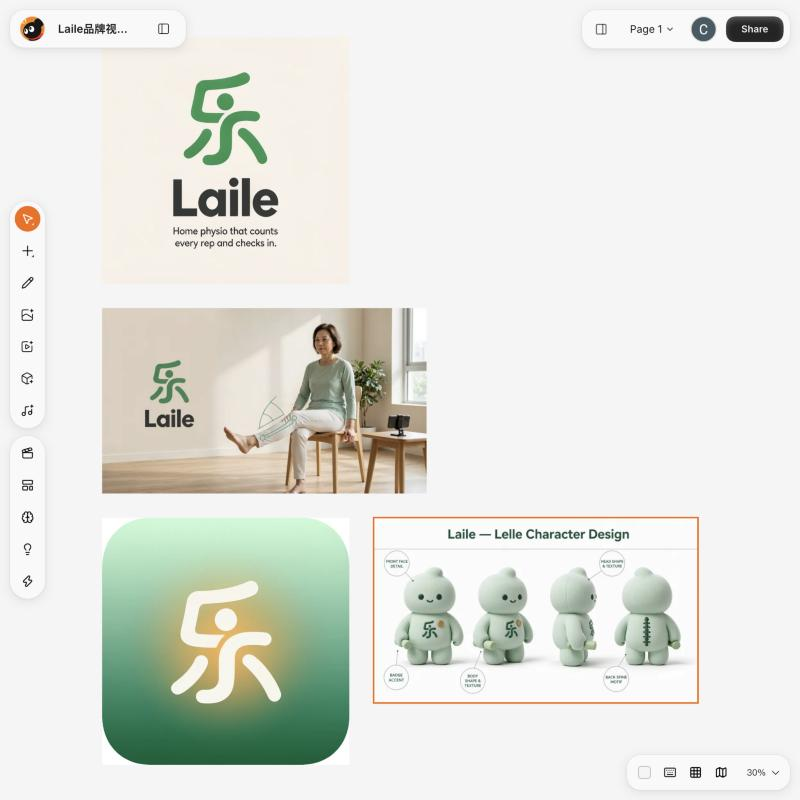
\includegraphics[width=0.95\linewidth]{../codebuddy/08-miora-brand-canvas.jpg}}\\[2pt]
  \capt{\textbf{Miora}: logo, cover, app icon, Lele mascot}
\end{column}
\begin{column}{0.30\textwidth}
  \centering
  \fbox{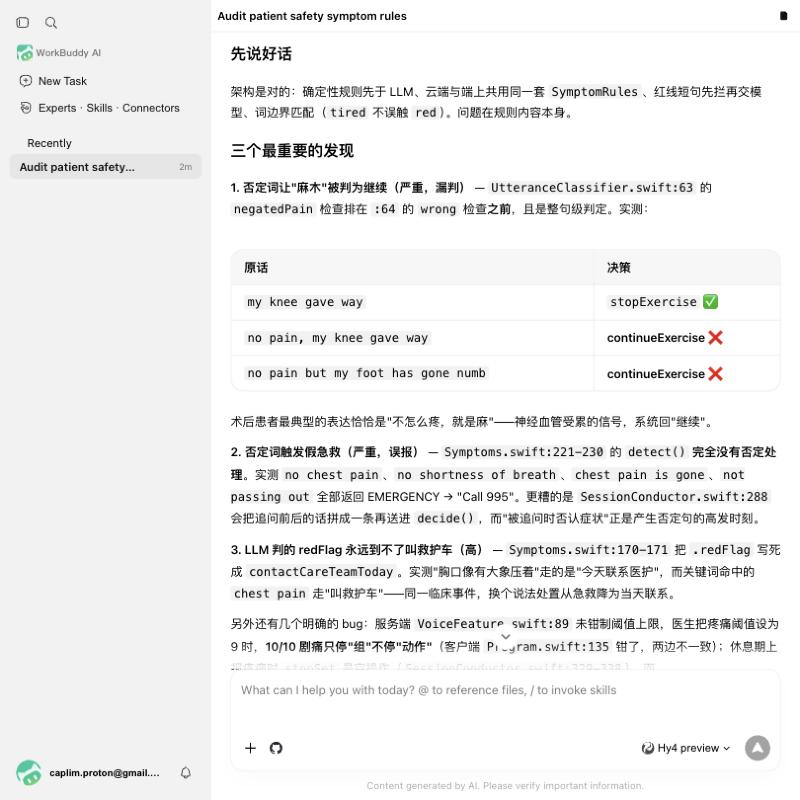
\includegraphics[width=0.95\linewidth]{../codebuddy/02-safety-audit-findings.jpg}}\\[2pt]
  \capt{\textbf{WorkBuddy}: safety audit with file and line findings}
\end{column}
\begin{column}{0.30\textwidth}
  \centering
  \fbox{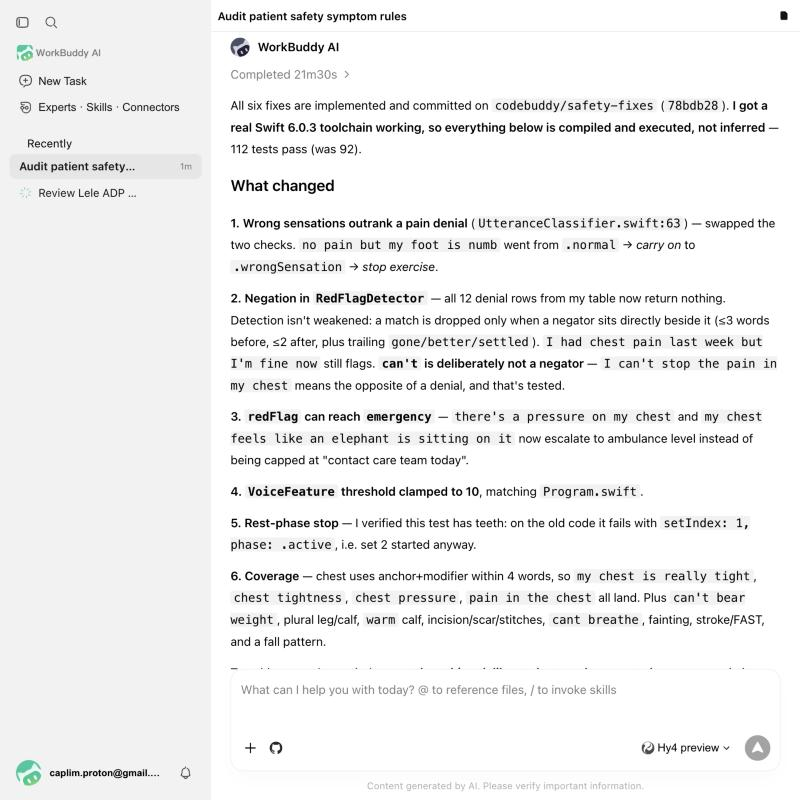
\includegraphics[width=0.95\linewidth]{../codebuddy/06-safety-fixes-done.jpg}}\\[2pt]
  \capt{\textbf{WorkBuddy}: six safety fixes, 112 tests passing}
\end{column}
\end{columns}
\vspace{6pt}
\begin{itemize}
  \item \textbf{CodeBuddy} found that ``no pain but my foot is numb'' was answered with ``carry on'' and that ``I haven't taken it yet'' was logged as a dose; its fixes were reviewed and merged.
  \item \textbf{ADP} runs Lele (chat, drafts, physio summaries); \textbf{Lighthouse} hosts the server, web app and portal.
\end{itemize}
\end{frame}

% ---- 10. Fit ------------------------------------------------------------
\begin{frame}{Fit with Challenge 2}
\small
\begin{tabularx}{\linewidth}{@{}>{\raggedright\arraybackslash}p{4.2cm}X@{}}
\toprule
Medication understanding & ``What's this for?'' on every dose, from the medicines knowledge base\\
Medication management & Reminders at the doctor's times; one tap or a typed reply marks a dose taken\\
Adherence support & Camera-verified sessions, check-in targets, forgiving streaks, barrier questions, new plans by chat\\
Health tracking & Knee bend, straightening gap, arm lift, reps, holds and pain against baseline\\
Preventive health & Precautions follow you; plateau and missed-day flags; follow-on programs\\
Healthcare preparation & Visit prep questions; pre-visit report and Lele's summary for the physio\\
Safe, bounded, honest & Rule-based red flags and referrals; no count without a clear view\\
\bottomrule
\end{tabularx}
\end{frame}

% ---- 11. Business --------------------------------------------------------
\begin{frame}{Why it can last}
\begin{columns}[t]
\begin{column}{0.48\textwidth}
  \textbf{\color{accent}Clinics}\\
  Verified adherence, live sessions and a prioritised daily list without extra visits. Proposed: a monthly fee per active patient.\\[10pt]
  \textbf{\color{accent}People}\\
  Discharge leads to a calisthenics or mobility program with limits carried over. Consumer subscription for people without a physio.
\end{column}
\begin{column}{0.48\textwidth}
  \textbf{\color{accent}A loop}\\
  Everyday users with aches are pointed to a physio; physio patients become everyday users afterwards.\\[10pt]
  \textbf{\color{accent}Cheap to run}\\
  Pose estimation on the device; model calls only for conversation, drafts and briefs; voice lines cached and paid for once.
\end{column}
\end{columns}
\end{frame}

% ---- 12. Status ---------------------------------------------------------
\begin{frame}{Where it stands}
\begin{columns}[t]
\begin{column}{0.48\textwidth}
  \textbf{\color{accent}Working now}
  \begin{itemize}
    \item iOS app on TestFlight with a public link
    \item Web app with webcam sessions, no install
    \item Server, portal and web app on Tencent Cloud Lighthouse
    \item Lele on Tencent Cloud ADP: chat, plans, physio summaries
    \item Camera pipeline tested with simulated skeletons
    \item 166 automated tests
  \end{itemize}
\end{column}
\begin{column}{0.48\textwidth}
  \textbf{\color{accent}Next}
  \begin{itemize}
    \item TencentDB for PostgreSQL
    \item Testing with people at home: camera placement, lighting, voice across a room
    \item Knowledge base review by a physiotherapist and a pharmacist
    \item Pilot with one clinic
  \end{itemize}
\end{column}
\end{columns}
\vfill
{\small\color{muted}Source: github.com/LimCharles/laile \ \textbullet\ \ Try Lele: \href{https://adp.tencentcloud.com/webim_exp/\#/chat/nZbZZz}{adp.tencentcloud.com/webim\_exp/\#/chat/nZbZZz}\\ Portal: \href{https://43-156-108-79.sslip.io/portal}{43-156-108-79.sslip.io/portal} (clinician@laile.demo / laile-demo-2026)\\ Web app: \href{https://43-156-108-79.sslip.io/app}{43-156-108-79.sslip.io/app} \ \textbullet\ \ iPhone app: \href{https://testflight.apple.com/join/WuymKzUH}{testflight.apple.com/join/WuymKzUH}}
\end{frame}

% ---- 13. References ------------------------------------------------------
\begin{frame}{References}
\scriptsize
\begin{itemize}
  \item[{[1]}] Argent R, Daly A, Caulfield B. Patient involvement with home-based exercise programs: can connected health interventions influence adherence? \emph{JMIR mHealth uHealth} 2018;6(3):e47.
  \item[{[2]}] Jack K, McLean SM, Moffett JK, Gardiner E. Barriers to treatment adherence in physiotherapy outpatient clinics: a systematic review. \emph{Manual Therapy} 2010;15(3):220-228.
  \item[{[3]}] National Population and Talent Division. \emph{Population in Brief 2026}. Singapore, September 2026.
\end{itemize}
\end{frame}

\end{document}
